%Fred's NSF Grant Dec 2018
\documentclass[11pt]{NSFamsart}
\usepackage{latexsym,amsfonts,amsmath,epsfig,extdash,multirow}
\usepackage{stackrel,tabularx,mathtools,enumitem,xspace}
\usepackage[dvipsnames]{xcolor}
\usepackage[numbers]{natbib}
\usepackage{hyperref,accents, booktabs}
\usepackage{algorithm, algorithmic}
\usepackage{cleveref}
\newcommand{\myshade}{85}
\colorlet{mylinkcolor}{violet}
\colorlet{mycitecolor}{Aquamarine}
%\colorlet{mycitecolor}{OliveGreen}
\colorlet{myurlcolor}{YellowOrange}

\hypersetup{
	linkcolor  = mylinkcolor!\myshade!black,
	citecolor  = mycitecolor!\myshade!black,
	urlcolor   = myurlcolor!\myshade!black,
	colorlinks = true,
}


% This package prints the labels in the margin
%\usepackage[notref,notcite]{showkeys}


%\pagestyle{empty}
\thispagestyle{plain}
\pagestyle{plain}

\headsep-0.6in
%\headsep-0.45in

%%list of acronyms with links
\newcommand{\GAIL}{\hyperlink{GAILlink}{GAIL}\xspace}
\newcommand{\QMC}{\hyperlink{QMClink}{QMC}\xspace}
\newcommand{\IIDMC}{\hyperlink{IIDMClink}{IID MC}\xspace}
\newcommand{\SAMSIQMC}{\hyperlink{SAMSIlink}{SAMSI-QMC}\xspace}

\setlength{\textwidth}{6.4in}
\setlength{\oddsidemargin}{0in}
\setlength{\evensidemargin}{0in}
\textheight8.9in
%\textheight9.1in


\providecommand{\FJHickernell}{Hickernell}
\newcommand{\hf}{\widehat{f}}
\newcommand{\hI}{\hat{I}}
\newcommand{\hatf}{\hat{f}}
\newcommand{\hatg}{\hat{g}}
\newcommand{\tf}{\widetilde{f}}
\newcommand{\tbf}{\tilde{\bff}}
%\DeclareMathOperator{\Pr}{\mathbb{P}}
\DeclareMathOperator{\cost}{cost}
\DeclareMathOperator{\comp}{comp}

\DeclareMathOperator{\loss}{loss}
\DeclareMathOperator{\lof}{lof}
\DeclareMathOperator{\reg}{reg}
\DeclareMathOperator{\CV}{CV}
\DeclareMathOperator{\size}{wd}
\DeclareMathOperator{\GP}{\mathcal{G} \! \mathcal{P}}
\DeclareMathOperator{\erf}{erf}


\newcommand{\reals}{{\mathbb{R}}}
\newcommand{\naturals}{{\mathbb{N}}}
\newcommand{\natzero}{{\mathbb{N}_0}}
\newcommand{\integers}{{\mathbb{Z}}}
\def\expect{{\mathbb{E}}}
\def\il{\left<}
\def\ir{\right>}
\def\e{\varepsilon}
\def\g{\gamma}
\def\l{\lambda}
\def\b{\beta}
\def\a{\alpha}
\def\lall{\Lambda^{{\rm all}}}
\def\lstd{\Lambda^{{\rm std}}}

\newcommand{\vf}{\boldsymbol{f}}
\newcommand{\hV}{\widehat{V}}
\newcommand{\tV}{\widetilde{V}}
\newcommand{\fu}{\mathfrak{u}}
\newcommand{\hcut}{\mathfrak{h}}
\newcommand{\tOmega}{\widetilde{\Omega}}
\newcommand{\tvarrho}{\widetilde{\varrho}}

\newcommand{\bbE}{\mathbb{E}}
\newcommand{\tQ}{\widetilde{Q}}
\newcommand{\mA}{\mathsf{A}}
\newcommand{\mB}{\mathsf{B}}
\newcommand{\mC}{\mathsf{C}}
\newcommand{\mD}{\mathsf{D}}
\newcommand{\mG}{\mathsf{G}}
\newcommand{\mH}{\mathsf{H}}
\newcommand{\mI}{\mathsf{I}}
\newcommand{\bbK}{\mathbb{K}}
\newcommand{\mK}{\mathsf{K}}
\newcommand{\tmK}{\widetilde{\mathsf{K}}}
\newcommand{\mL}{\mathsf{L}}
\newcommand{\mM}{\mathsf{M}}
\newcommand{\mP}{\mathsf{P}}
\newcommand{\mQ}{\mathsf{Q}}
\newcommand{\mR}{\mathsf{R}}
\newcommand{\mX}{\mathsf{X}}
\newcommand{\mPhi}{\mathsf{\Phi}}
\newcommand{\mPsi}{\mathsf{\Psi}}
\newcommand{\mLambda}{\mathsf{\Lambda}}
\newcommand{\cube}{[0,1]^d}
\newcommand{\design}{\{\bx_i\}_{i=1}^n}

\DeclareMathOperator{\err}{err}
\DeclareMathOperator{\oerr}{\overline{\err}}
\DeclareMathOperator{\herr}{\widehat{\err}}
\DeclareMathOperator{\Ans}{Ans}

\DeclareMathOperator{\Var}{Var}
\DeclareMathOperator{\SOL}{SOL}
\DeclareMathOperator{\APP}{APP}
\DeclareMathOperator{\ALG}{ALG}
\DeclareMathOperator{\OPER}{OPER}



\DeclareMathOperator{\INT}{INT}
\DeclareMathOperator{\OPT}{MIN}

\newcommand{\bone}{\boldsymbol{1}}
\newcommand{\bzero}{\boldsymbol{0}}
\newcommand{\binf}{\boldsymbol{\infty}}
\newcommand{\ba}{{\boldsymbol{a}}}
\newcommand{\bb}{{\boldsymbol{b}}}
\newcommand{\bc}{{\boldsymbol{c}}}
\newcommand{\bd}{{\boldsymbol{d}}}
\newcommand{\be}{{\boldsymbol{e}}}
\newcommand{\bff}{{\boldsymbol{f}}}
\newcommand{\bhh}{{\boldsymbol{h}}}
\newcommand{\beps}{{\boldsymbol{\varepsilon}}}
\newcommand{\tbeps}{\tilde{\beps}}
\newcommand{\bx}{{\boldsymbol{x}}}
\newcommand{\bX}{{\boldsymbol{X}}}
\newcommand{\bh}{{\boldsymbol{h}}}
\newcommand{\bk}{{\boldsymbol{k}}}
\newcommand{\bg}{{\boldsymbol{g}}}
\newcommand{\bn}{{\boldsymbol{n}}}
\newcommand{\bv}{{\boldsymbol{v}}}
\newcommand{\bu}{{\boldsymbol{u}}}
\newcommand{\by}{{\boldsymbol{y}}}
\newcommand{\bt}{{\boldsymbol{t}}}
\newcommand{\bz}{{\boldsymbol{z}}}
\newcommand{\bvarphi}{{\boldsymbol{\varphi}}}
\newcommand{\bgamma}{{\boldsymbol{\gamma}}}
\newcommand{\bphi}{{\boldsymbol{\phi}}}
\newcommand{\bpsi}{{\boldsymbol{\psi}}}
\newcommand{\bnu}{{\boldsymbol{\nu}}}
\newcommand{\balpha}{{\boldsymbol{\alpha}}}
\newcommand{\bbeta}{{\boldsymbol{\beta}}}
\newcommand{\bo}{{\boldsymbol{\omega}}}  %GF added
\newcommand{\newton}[2]{\left(\begin{array}{c} #1\\ #2\end{array}\right)}
\newcommand{\anor}[2]{\| #1\|_{\mu_{#2}}}
\newcommand{\satop}[2]{\stackrel{\scriptstyle{#1}}{\scriptstyle{#2}}}
\newcommand{\setu}{{\mathfrak{u}}}

\newcommand{\me}{\textup{e}}
\newcommand{\mi}{\textup{i}}
\def\d{\textup{d}}
\def\dif{\textup{d}}
\newcommand{\cc}{\mathcal{C}}
\newcommand{\cb}{\mathcal{B}}
\newcommand{\cl}{L}
\newcommand{\ct}{\mathfrak{T}}
\newcommand{\cx}{{\Omega}}
\newcommand{\calc}{{\mathcal{C}}}
\newcommand{\calf}{{\mathcal{F}}}
\newcommand{\calfd}{{\calf_d}}
\newcommand{\calh}{{\mathcal{H}}}
\newcommand{\tcalh}{{\widetilde{\calh}}}
\newcommand{\calI}{{\mathcal{I}}}
\newcommand{\calhk}{\calh_d(K)}
\newcommand{\calg}{{\mathcal{G}}}
\newcommand{\calgd}{{\calg_d}}
\newcommand{\cL}{\mathcal{L}}
\newcommand{\cP}{\mathcal{P}}
\newcommand{\cT}{\mathcal{T}}
\newcommand{\cK}{\mathcal{K}}
\newcommand{\fA}{\mathfrak{A}}
\newcommand{\fC}{\mathfrak{C}}
\newcommand{\fF}{\mathfrak{F}}
\newcommand{\fL}{\mathfrak{L}}
\newcommand{\fU}{\mathfrak{U}}
\newcommand{\hS}{\widehat{S}}
\DeclareMathOperator{\Prob}{\mathbb{P}}

\def\abs#1{\ensuremath{\left \lvert #1 \right \rvert}}
\newcommand{\bigabs}[1]{\ensuremath{\bigl \lvert #1 \bigr \rvert}}
\newcommand{\norm}[2][{}]{\ensuremath{\left \lVert #2 \right \rVert}_{#1}}
\newcommand{\ip}[3][{}]{\ensuremath{\left \langle #2, #3 \right \rangle_{#1}}}
\newcommand{\bignorm}[2][{}]{\ensuremath{\bigl \lVert #2 \bigr \rVert}_{#1}}
\newcommand{\calm}{{\mathfrak{M}}}
\DeclareMathOperator{\diag}{diag}
\DeclareMathOperator{\dist}{dist}
\DeclareMathOperator{\filldis}{fill}
\DeclareMathOperator{\sep}{sep}
\DeclareMathOperator{\avg}{avg}
\DeclareMathOperator{\vol}{vol}
\DeclareMathOperator{\cov}{cov}

\newcommand{\des}{\{\bx_i\}}
\newcommand{\desinf}{\{\bx_i\}_{i=1}^{\infty}}
\newcommand{\desn}{\{\bx_i\}_{i=1}^n}
\newcommand{\wts}{\{g_i\}_{i=1}^N}
\newcommand{\wtsn}{\{g_i\}_{i=1}^N}
\newcommand{\datan}{\{y_i\}_{i=1}^N}

%FJH added
\newcommand{\Order}{\mathcal{O}}
\newcommand{\ch}{\mathcal{H}}
\newcommand{\tch}{{\widetilde{\ch}}}
\newcommand{\veps}{\boldsymbol{\varepsilon}}
\DeclareMathOperator{\best}{best}
\newcommand{\hmu}{\hat{\mu}}
\newcommand{\hsigma}{\hat{\sigma}}
\newcommand{\tK}{\widetilde{K}}
\newcommand{\Matlab}{{\sc Matlab}\xspace}
\newcommand{\abstol}{\varepsilon_{\text{a}}}
\newcommand{\reltol}{\varepsilon_{\text{r}}}

\newcommand\starred[1]{\accentset{\star}{#1}}


\definecolor{MATLABOrange}{rgb}{0.85,  0.325, 0.098}

%\newtheorem{resproblem}{Research Problem}
%\newtheorem{research}{Research Objectives}



%\setcounter{page}{1}

\setlist[description]{font=\normalfont\itshape}



\begin{document}
%\setlength{\leftmargini}{2.5ex}

\centerline{\Large \textbf{Project Description}}
\vspace{-2ex}

\setcounter{tocdepth}{1}
\tableofcontents

\vspace{-6ex}

\section{Scientific Context, Key Ideas,  and Timeliness of the Proposed Research}
Integration and function approximation are the nuts and bolts when 
solving practical problems in a variety of areas, including financial risk management \cite{Gla03}, 
statistical physics~\cite{LanBin14}, 
Bayesian inference~\cite{GelEtal13}, and uncertainty quantification~\cite{ForEtal09, Smi14a}.  As computational mathematicians, we should aim to provide algorithms that meet the needs of practitioners.  They want algorithms that 
\begin{enumerate}[leftmargin = 15ex]
\renewcommand{\labelenumi}{\textbf{Goal \arabic{enumi}.}}
    \item \label{GoalOne} Expend the  
computational effort required to meet their error criterion, but do not expend much more effort;
\item Require minimal a priori knowledge about the input function;

\item Are computationally efficient; and

\item Are readily available and easy to use.
\end{enumerate}
We propose to construct algorithms that meet those goals.

\subsubsection*{Problems to be Solved} The mathematical problems that we wish to solve take the form 
\begin{subequations} \label{problem}
\begin{align}
    \calf & = \text{a Banach space of inputs}, \qquad 
    \calg = \text{a Banach space of outputs} \\
    \SOL : \calf  \to \calg & = \text{ a linear solution operator} \\
    \nonumber
    & \qquad \text{e.g., integration }\SOL(f) := \int_{\cube} f(\bx) \, \dif \bx \\
    \nonumber
    & \qquad \text{or function approximation } \SOL(f) = f.
\end{align}
\end{subequations}
There exist approximate solutions requiring $n$ function values at well-chosen node sets, $\design$, which take the form
\begin{equation}
    \APP: \calf \times \naturals_0 \to \calg = \text{fixed sample size approximation}, \quad \APP(f,n) = \sum_{i=1}^n f(\bx_i) g_i.
\end{equation}
For integration, the $g_i$ are real-valued weights, which are generally equal for (quasi\Hyphdash*)Monte Carlo methods but unequal for Newton-Cotes or Gaussian quadrature rules.  For function approximation, the $g_i$ are called cardinal functions. Since our solution operator is linear, it is natural to consider approximations that are also linear.  We define $\APP(f,0) = 0$.

To meet Goal \ref{GoalOne} we need to bound the error of our approximations.  Error bounds often take the form of 
\begin{subequations} \label{errorBd}
\begin{gather} 
    \norm[\calg]{\SOL(f) - \APP(f,n)} \le \norm[\calf \to \calg]{\SOL(\cdot) - \APP(\cdot,n)} \, \norm[\calf]{f}, \qquad \forall f\in \calf, \ n \in \natzero, \\
    \intertext{where the norm of a linear operator $\OPER : \calf \to \calg$ is defined as}
    \norm[\calf \to \calg]{\OPER(\cdot)} : = \sup_{f \in \calf, \ f \ne 0} \frac{ \norm[\calg]{\OPER(f)}}{\norm[\calf]{f}}.
\end{gather}
\end{subequations}
Here, $\norm[\calf]{\cdot}$ is a (semi-)norm.  E.g., for the composite trapezoidal rule one may choose $\norm[\calf]{f}$ to be the total variation of $f'$, in which case $\norm[\calf \to \calg]{\SOL(\cdot) - \APP(\cdot,n)} = 1/[8 (n-1)^2]$ \cite[Sect.\ 7.2, (7.15)]{BraPet11a}.  Even if the norm of the error operator has an explicit expression or upper bound, $\norm[\calf]{f}$ is typically unknown a priori.  Therefore, error bound \eqref{errorBd} is insufficient to satisfy Goal \ref{GoalOne}. 

\subsubsection*{Adaptive Algorithms} Goal \ref{GoalOne} requires an algorithm of the form
\begin{subequations} \label{AlgErr}
\begin{gather}
    \ALG(f,\varepsilon) : \calf \times (0,\infty) \to \calg = \text{fixed tolerance algorithm},
    \intertext{which satisfies}
    \norm[\calg]{\SOL(f) - \ALG(f,\varepsilon)} \le \varepsilon \quad \text{(with high probability)} \qquad \forall f\in \calc, \ \varepsilon >0,
\end{gather}
\end{subequations}
where $\calc$ is a well-chosen subset of $\calf$ for which $\ALG$ can be proven to succeed.  This means that the user need only specify the error tolerance, $\varepsilon$, and is freed from having to choose the appropriate $n$.  The computational cost is determined by the accuracy requirement.  If the algorithm is random, we are willing to accept that it satisfies the error tolerance with high probability rather than all the time.  

Algorithms satisfying \eqref{AlgErr} use approximations satisfying \eqref{errorBd} combined with a \emph{stopping criterion} that adaptively determines the necessary $n$.  As candidates for $n$ increase, $\ALG$ must rely on the definition of $\calc$ plus the function values sampled to obtain $\APP(f,n)$ to reliably bound the error $\norm[\calg]{\SOL(f) - \APP(f,n)}$ and determine whether $n$ is large enough.

While there is a substantial literature on approximations satisfying \eqref{errorBd}, the work required construct a stopping criterion needed to obtain the algorithm satisfying \eqref{AlgErr} has been neglected.  For simpler problems, such as evaluating elementary and even special functions,
\begin{equation} \label{functionValues}
    \sin, \cos, \exp, \log, \erf, \text{ the (inverse) Gaussian CDF, Bessel functions, etc.}
\end{equation}
we already have trustworthy algorithms.
For these problems, $\calf$ and $\calg$ are subsets of real numbers, and we understand well the potential pitfalls of representing these numbers in finite precision.

However, for integration and function approximation, the inputs are functions, for which we only have partial information---function values at a finite number of points.  Therefore, satisfying Goal \ref{GoalOne} is more difficult for these problems than it is for problems of the form \eqref{functionValues}.  

\subsubsection*{Existing Adaptive Algorithms Typically Employ Heuristic Stopping Criteria}
The demand for algorithms satisfying Goal \ref{GoalOne} is evidenced by the automatic quadrature, function approximation, and optimization routines found in general purpose software.  For example, MATLAB default integration routine, 
\texttt{integral} \cite{MAT9.3}, is based on \cite{Sha08a}, and estimates the error based on the difference between two different quadratures that use the same nodes. Over 30 years ago, James 
Lyness \cite[p.\ 69]{Lyn83} pointed out the flaws in this and nearly all adaptive quadratures:
\begin{quote}
	While prepared to take the risk of being misled by chance alignment of zeros in the integrand 
	function, or by narrow peaks which are ``missed,'' the user may wish to be reassured that for 
	``reasonable'' integrand functions which do not have these characteristics all will be well. It is the 
	purpose of the rest of this section to demonstrate by example that he cannot be reassured on this 
	point. In fact the routine is likely to be unreliable in a significant proportion of the problems it faces 
	(say $1$ to $5\%$) and there is no way of predicting in a straightforward way in which of any set 
	of apparently reasonable problems this will happen.
\end{quote}

\begin{figure}[h]
	\begin{tabular}{>{\centering}m{0.31\textwidth}@{\quad}>{\centering}m{0.31\textwidth}@{\quad}>{\centering}m{0.3\textwidth}}
		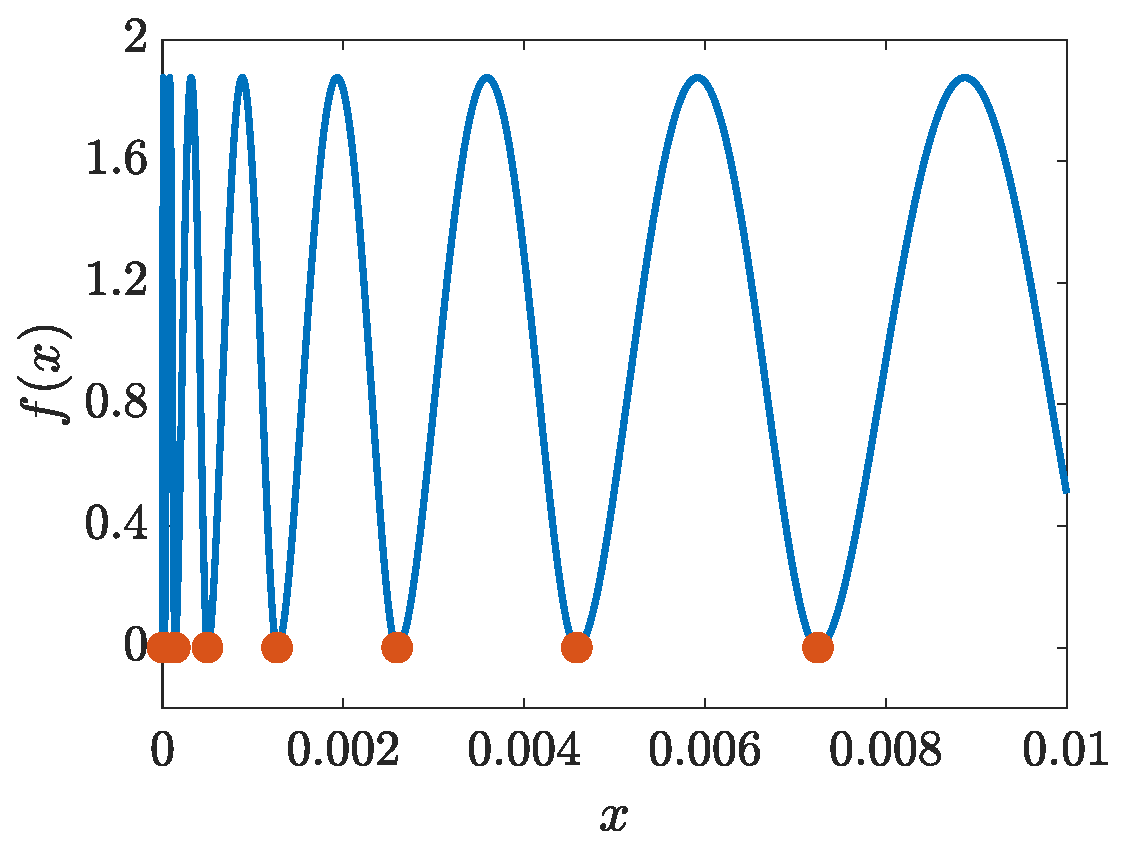
\includegraphics[width=0.3\textwidth]{ProgramsImages/SpikyFoolIntegralcolor.eps} &
		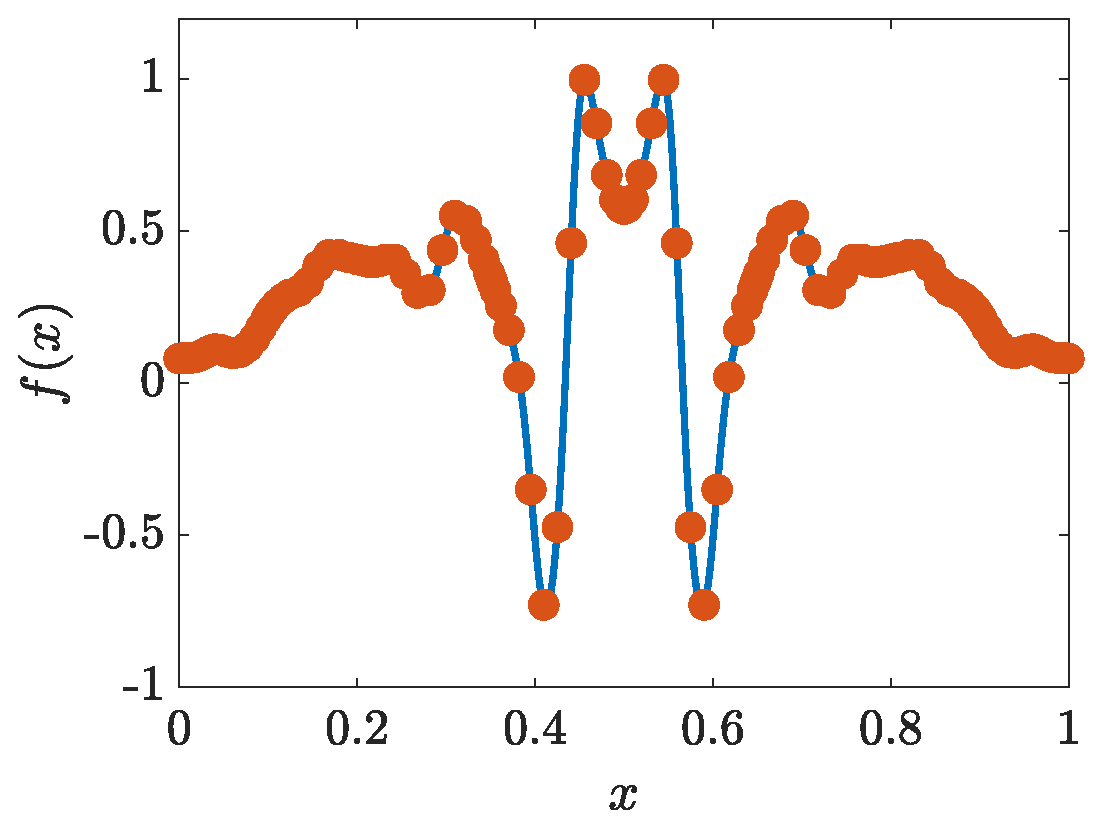
\includegraphics[width=0.3\textwidth]{ProgramsImages/FlukyFoolIntegralcolor.eps} 
		\tabularnewline
		(a) $\err_{100}(f) = 1 $ &
		(b) $\err_{100}(f) =  1.4\text{E}{-4}$ &
		(c) $\err_{150}(f) =  2.8\text{E}{-5}$
		\end{tabular}
	\caption{Integrands for which $\herr_n(f) = 0$ but 
	$\err_n(f) \ne 0$. \label{quadfailfig}}
\end{figure}




======================

======================




The desire for algorithms satisfying Goal \ref{GoalOne} is evidenced by the automatic quadrature, function approximation, and optimization routines found in general purpose software.  


It is impossible to expect fixed tolerance algorithm to be successful for all $f \in \calf$ unless As will be explained later




Practitioners 
want to expend the  
computational effort required to meet their error criterion, but not much more. 
Practitioners also want the algorithm to require no more than the problem specification and the 
error criterion.   Adaptive algorithms fill this need by determining when to stop the computation 
based on data-driven error bounds, $\herr_n(f)$, where $f$ is the input function and $n$ is the 
number of nodes (points where $f$ is evaluated).



Common adaptive algorithms employ \emph{heuristic} error bounds, that sometimes fail, and fail for 
unknown reasons. Traditional error 
analysis for numerical algorithms 
yields rigorous error bounds, $\oerr_n(f)$, which involve norms of the input functions, 
$\norm[\calf]{f}$.  However, $\norm[\calf]{f}$ is typically unknown a 
priori.  Thus, traditional  error 
bounds alone are inadequate  to produce rigorous stopping criteria for adaptive algorithms.

Our project will develop \emph{rigorous} data-driven error bounds that will underpin new adaptive 
numerical algorithms for integration and function approximation.  The 
key---discovered in our recent NSF-funded research---is to identify a cone of \emph{reasonable} 
input functions, 
$\cc$,  for which the traditional error bounds can certainly be bounded in terms of 
data-driven error bounds, i.e., $\oerr_n(f) \le \herr_n(f)$ for all $f \in \cc$.  To guarantee their 
correctness, our data-driven error bounds typically are different than the heuristics commonly 
employed.
Our new adaptive algorithms will yield answers with the desired accuracy and require only 
specification of the problem and the error tolerance---not a bound on $\norm[\calf]{f}$. 
These adaptive algorithms will be implemented in our freely available \GAIL software library.  They 
will 
be tested on various applications problems to ensure that theory matches practice.  The 
development, implementation and application of these algorithms will involve high school 
students through senior faculty in a variety of disciplines.

\subsection{An Illustrative Example: Integration by the Trapezoidal Rule}  
\label{TrapIllSect}
We introduce some 
key ideas in our proposed research via the problem of univariate integration.  Calculus 
students are taught to approximate the definite integral by the trapezoidal rule 
\cite[Sect.\ 7.2, (7.15)]{BraPet11a}:
\begin{gather}
\label{traprule}
\int_0^1 f(x) \, \dif x \approx T_n(f):= \frac1{2n} \left[f(0) + 2f(1/n) + \cdots + 2f(1-1/n) + f(1) \right ], \\
\label{traperrbd}
\err_n(f) := \abs{\int_0^1 f(x) \, \dif x - T_n(f)}  \le \frac{\Var(f')}{8 n^2} =: \oerr_n(f),
\end{gather}
where the total variation of the first derivative is defined as 
\begin{equation*}
\Var(f') : = \sup \left \{\widehat{V}(f',\{t_i\}_{i=0}^n) := \sum_{i=2}^{n-1}  \abs{f'(t_i) - f'(t_{i-1})} \, \Big 
\vert \, 
\forall \text{ partitions }  \{t_i\}_{i=0}^n \text{ of } [0,1], \ \forall n \in \naturals \right \}.
\end{equation*} 
A partition of an interval is an ordered subset including both endpoints.
The practitioner wants to know how large $n$ 
must be to ensure that $\err_n(f)  \le \varepsilon$ for a prescribed 
absolute error tolerance $\varepsilon$.  Ensuring that $\oerr_n(f) \le \varepsilon$ is sufficient, but 
this requires an upper bound on $\Var(f')$, which is normally unavailable  unless $f$ has a simple 
form.

Numerical analysis texts  \cite[p.\ 223--224]{BurFai10}, \cite[p.\ 233]{CheKin12a}, 
and  \cite[p.\ 270]{Sau12a} propose estimating the absolute error of $T_n(f)$ by 
\begin{equation} \label{tradtraperrest}
 \err_n(f) \approx  \abs{\frac{T_n(f) - T_{n/2}(f)}{3}} =: \herr_n(f).
\end{equation}
Although this $\herr_n(f)$ is valid in some cases, it is flawed.  This $\herr_n(f)$  fails for 
spiky integrands whose 
spikes fall  between the nodes as in Figure \ref{quadfailfig}(a).  Worse, this $\herr_n(f)$ can fail 
for 
integrands that are \emph{not spiky} if $T_n(f)$ is coincidentally (nearly) 
the same as  $T_{n/2}(f)$ (see Figure \ref{quadfailfig}(b)).  Over 30 years ago, James 
Lyness \cite[p.\ 69]{Lyn83} pointed out the flaws of nearly all adaptive quadratures:
\begin{quote}
	While prepared to take the risk of being misled by chance alignment of zeros in the integrand 
	function, or by narrow peaks which are ``missed,'' the user may wish to be reassured that for 
	``reasonable'' integrand functions which do not have these characteristics all will be well. It is the 
	purpose of the rest of this section to demonstrate by example that he cannot be reassured on this 
	point. In fact the routine is likely to be unreliable in a significant proportion of the problems it faces 
	(say $1$ to $5\%$) and there is no way of predicting in a straightforward way in which of any set 
	of apparently reasonable problems this will happen.
\end{quote}
Figure \ref{quadfailfig}(b) depicts a reasonable integrand for which $\herr_n(f)$ in 
\eqref{tradtraperrest} fails.  Figure 
\ref{quadfailfig}(c) depicts a reasonable integrand for which the error estimate, $\herr_n(f)$, 
used 
by  
MATLAB's adaptive quadrature 
\texttt{integral} \cite{MAT9.3} fails.  

\begin{figure}[h]
	\begin{tabular}{>{\centering}m{0.31\textwidth}@{\quad}>{\centering}m{0.31\textwidth}@{\quad}>{\centering}m{0.3\textwidth}}
		\includegraphics[width=0.3\textwidth]{ProgramsImages/SpikyFoolTrapezoidalcolor.eps} &
		\includegraphics[width=0.3\textwidth]{ProgramsImages/FlukyFoolTrapezoidalcolor.eps} &
		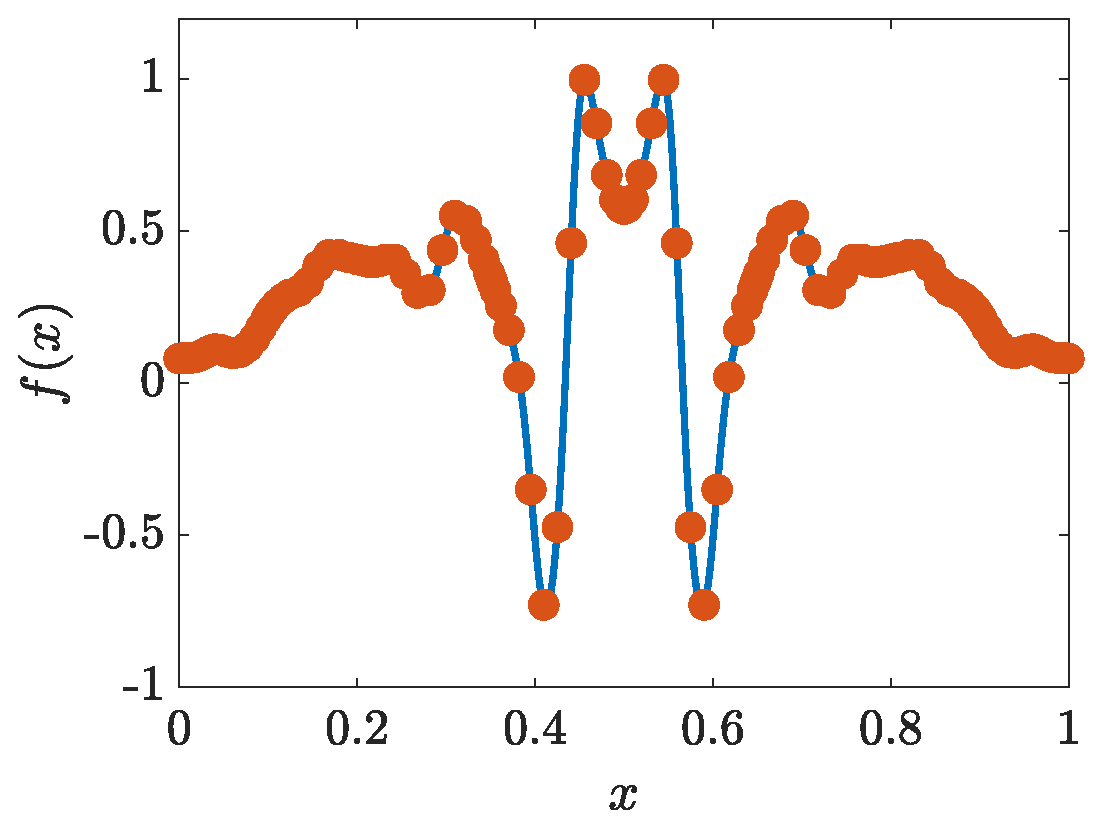
\includegraphics[width=0.3\textwidth]{ProgramsImages/FlukyFoolIntegralcolor.eps} 
		\tabularnewline
		(a) $\err_{100}(f) = 1 $ &
		(b) $\err_{100}(f) =  1.4\text{E}{-4}$ &
		(c) $\err_{150}(f) =  2.8\text{E}{-5}$
		\end{tabular}
	\caption{Integrands for which $\herr_n(f) = 0$ but 
	$\err_n(f) \ne 0$. \label{quadfailfig}}
\end{figure}

Despite Lyness's gloomy portrayal of adaptive quadratures, the PI and his collaborators have 
developed an adaptive trapezoidal algorithm that \emph{succeeds for all reasonable integrands}, 
although 
it 
may fail for spiky integrands \cite{HicEtal14a,HicRazYun15a}. The key is a 
data-based upper bound on $\Var(f')$.  

Here we outline the key arguments from \cite{HicRazYun15a}.  Let 
$\size(\{t_i\}_{i=0}^n) : = \max_{1 \le i \le n} t_i - t_{i-1}$ denote the partition width.  By 
definition, $\Var(f')$ is bounded below by $\widehat{V}(f',\{t_i\}_{i=0}^n)$ for any partition. 
Reasonable integrands are defined as those functions for which an inflated lower bound on  
$\Var(f')$ provides an \emph{upper bound} on $\Var(f')$:
\begin{multline} \label{conedef}
\cc := \Bigl \{ f \in C^1[0,1]: \Var(f') \le \fC(\size(\{t_i\}_{i=0}^n)) \hV(f',\{t_i\}_{i=0}^n) \text{ for all }   n 
\in \naturals \\
 \text{and partitions } \{t_i\}_{i=0}^n \text{ with } 
\size(\{t_i\}_{i=0}^n) < \hcut \Bigr \}, \qquad  \fC(h) := \frac{\fC_0 \hcut}{\hcut - h}, \quad \fC_0 
> 1, \ 
\ 0 < \hcut < 1.
\end{multline}
This set of reasonable integrands, $\cc$, is a \emph{cone} since $f \in \cc \implies cf \in \cc$ 
for 
any 
constant $c$.  The 
parameters $\hcut$ and $\fC_0$ determine how inclusive this 
cone of reasonable functions is.  It is shown in \cite{HicRazYun15a} that $\Var(f')$ can rigorously be 
bounded above by an 
inflated variation of the derivative of the linear spline, which depends only on function values, not on 
derivative values:
\begin{subequations} \label{tVdef}
\begin{gather} 
\tV_n(f) 
% & : = \sum_{i=1}^{n-1} \abs{ \frac{f((i+1)/n)-f(i/n)}{1/n} - \frac{f(i/n)-f((i-1)/n)}{1/n}}  \\& 
:= n\sum_{i=1}^{n-1} \abs{f((i+1)/n)-2f(i/n)+f((i-1)/n)}, 
\\ \Var(f') \le \fC(2/n) \tV_n(f),  \ \ 
\forall 
f \in \fC,  \ n > 2 /\hcut.
\end{gather}
\end{subequations}
This provides a data-driven upper bound on the error  of the trapezoidal rule, namely,
\begin{equation} \label{guartraperrest}
\err_n(f) \le \oerr_n(f) \le \herr_n(f) := \frac{\fC(2/n) \tV_n(f)}{8n^2} \qquad 
\forall 
f \in \fC,  \ n > 2 \hcut.
\end{equation}
An adaptive quadrature, Algorithm \ref{Trapalg},  is constructed by increasing $n$ until 
$\herr_n(f)$ does 
not exceed the error tolerance, $\varepsilon$.

\begin{algorithm}
	\caption{Adaptive Trapezoidal Rule \label{Trapalg}} 
	\begin{algorithmic}[1]
		\REQUIRE a black-box function, $f$; an absolute error tolerance,
		$\varepsilon>0$; the maximum partition width, $\hcut$; the constant $\fC_0 > 1$;  the 
		maximum number of trapezoids, $n_{\max}$

\ENSURE $\abs{\int_0^1 f(x) \dif x - \ct(f,\varepsilon)} \le \varepsilon$, provided $f \in \cc$

\STATE $n \leftarrow \lfloor 1 /\hcut \rfloor + 1$

\REPEAT

\STATE $n \leftarrow 2n$

\STATE Compute $\herr_n(f)$ according to \eqref{guartraperrest}

\UNTIL  $\herr_n(f) \le \varepsilon$ or $n > n_{\max}$

\STATE Compute $\ct(f,\varepsilon) = T_n(f)$ according to \eqref{traprule}.
		
\end{algorithmic}
	\end{algorithm}


\subsection{Key Ideas Illustrated by the Adaptive Trapezoidal Rule Algorithm 
\ref{Trapalg}} 
\label{subsect:trap}

\begin{description}[leftmargin=2.5ex]
	\item[Bound the error by bounding the semi-norm of $f$] Algorithm \ref{Trapalg} succeeds 
	by 
	\emph{bounding} 
	$\Var(f')$---a key term in 
	$\oerr_n(f)$ in \eqref{traperrbd}---for reasonable functions:
	\begin{equation*}
	\underbrace{\err_n(f)}_{\text{actual error}} \ \ \underbrace{\le}_{\text{all } f} \ \ 	
	\underbrace{\oerr_n(f)}_{\text{theoretical  bound}} \ \ \underbrace{\le}_{f \in \cc} \ \ 
	\underbrace{\herr_n(f)}_{\text{data-driven  bound}} .
	\end{equation*}
	Typical  adaptive quadrature 
	algorithms 
	remain 
	flawed because they assume that the difference between two quadrature rules is indicative of the 
	error of one of them as in \eqref{tradtraperrest}.  
	
	\item[Identify a cone, $\cc$, of reasonable functions] Our set of reasonable functions is a 
	\emph{cone} 
	defined precisely in \eqref{conedef}.  The widest spike must be wider than the minimum 
	width, $\hcut$.  
	The bound of $\Var(f')$ in terms of an inflated $ \hV(f',\{t_i\}_{i=0}^n)$ excludes functions with 
	large
	changes in $f'$ over small intervals.
	
	\item[$\cc$ is non-convex] A convex combination of two reasonable 
	functions, $f_1$ and 
	$f_2$, may produce 
	a spiky function as illustrated below (the narrow width, not the height makes it a spike):
	
	\centerline{\includegraphics[width = 0.35\textwidth]{ProgramsImages/broadpk.png}
	\includegraphics[width = 0.35\textwidth]{ProgramsImages/choppedpk.png}
\includegraphics[width = 0.35\textwidth]{ProgramsImages/narrowpk.png}}

\vspace{-4ex}
  \noindent A non-convex cone of input functions, $\cc$, is key to an adaptive algorithm 
  that outperforms non-adaptive algorithms.  For convex sets of input functions---such as 
  balls---adaptive algorithms have no 
  advantage under rather 
  general conditions  \cite[Chap.\ 4, Corollary 5.2.1]{TraWasWoz88}.
	

	\item[Bound the computational cost of the algorithm] Let $\cost(\ct,f,\varepsilon)$ denote the 
	computational cost or number of function values  required by 
	Algorithm \ref{Trapalg} to obtain $\ct(f,\varepsilon)$ for $f \in \cc$.  It is shown that 
	$\cost(\ct,f,\varepsilon) = \Order (\sqrt{\Var(f')/\varepsilon})$ in \cite{HicRazYun15a}.  
	(Since $\Var(f')$ is unbounded for $f \in \cc$, we 
	include it in the expression for the computational cost.)  The computational cost for Algorithm 
	\ref{Trapalg} is asymptotically the same as that for a non-adaptive trapezoidal rule when 
	$\Var(f')$ has a known 
	upper bound.  For 
	Algorithm \ref{Trapalg} an upper bound on $\Var(f')$ is \emph{not required}.
	
	\item[Show that the adaptive algorithm is optimal] The \emph{computational complexity} of this 
	integration problem is the computational cost of the best possible algorithm that is based on 
	function values only,  
	\[
	\comp(v,\varepsilon)  := \inf_ {\ct'} \ \sup\{\cost(\ct',f,\varepsilon) : f \in \cc, \Var(f') \le v \} .
	\]
	It is shown in \cite{HicRazYun15a} that $\comp(v,\varepsilon) = \Order 
	(\sqrt{v/\varepsilon})$ by constructing fooling functions that look like zero to the algorithm, but 
	whose 
	integral is nonzero. Our algorithm is asymptotically optimal.
	
	\item[The definition of adaptive algorithm includes parameters] MATLAB's 
	\texttt{integral} \cite{MAT9.3}
	assumes an initial number of nodes and a maximum sample size.  
	%Chebfun \cite{TrefEtal17a}, a numerical library that adaptively integrates functions via 
	%Chebyshev polynomial approximations assumes default values for these parameters as well as 
	%others.
	These parameters are set to be reasonable for most situations, but may be modified if 
	necessary.  The parameters  $\hcut = 0.02, \fC_0 = 
	1.5$, and 
	$n_{\max} = 10^7$ are meant to remain the same from problem to problem, but may be 
	modified 
	to 
	enhance speed or increase robustness.
	
	\item[The adaptive algorithm is available]  Algorithm 1 and related adaptive algorithms 
	developed 
	by the PI and his collaborators have been published in the Guaranteed Automatic 
	Integration 
	Library (\hypertarget{GAILlink}{GAIL}) \cite{ChoEtal17b}.  We propose to further develop this 
	library (Sect.\ 
	\ref{BroaderTwoSec}).
	
	\item[An error bound exists even if  time is the limiting factor]  Specifying the number of 
nodes rather than the error tolerance is accomplished by setting $n_{\max}$ to be this
 number and $\varepsilon = 0$.  The error bound, $\herr_n(f)$, is not needed to 
stop the algorithm but is available to inform the user how large the error might be.

	\item[This algorithm is globally adaptive] The  quadrature algorithm 
	described above adaptively determines $n$ based on function data, which we term \emph{global 
	adaptivity}.  Algorithms that determine the pattern of the nodes---as well as their number---based 
	on function data are termed \emph{locally adaptive}.  Sect.\ 
	\ref{previousmeritsubsec} describes new locally adaptive algorithms.
	
	\item[Optimality is only for integrands with limited smoothness] This adaptive quadrature 
	algorithm is 
	optimal for the cone of integrands, $\cc$, however, it is 
	sub-optimal for smoother integrands.  See Sect.\ \ref{SectUniProb} for proposed research on 
	algorithms with
	higher order convergence.
	
\end{description}

Our proposed research addresses problems beyond just univariate integration.  The next 
subsections provide the notation for these problems and outline our research goals.


\subsection{Traditional Error Analysis} Let $\calf$ be a Banach space of input functions 
defined on the domain $\cx$, let
$\calg$ be a Banach space of possible 
solutions, and let $S:\calf \to \calg$ be a solution operator.  Some examples of solution 
operators for integration, function approximation, and optimization are
\begin{equation} \label{probs}
S = \INT: f \mapsto \int_{\Omega} f(\bx) \, \dif \bx, \qquad S = \APP:f \mapsto f, \qquad S = 
\OPT :f \mapsto 
\min_{\bx \in \Omega} f(\bx).
% \\S: f \mapsto u, \text{ where } u'' + u = f(x), \quad u(0) = u(1) = 0.
\end{equation}
Let $\{A_n: 
\calf \to \calg\}_{n \in \calI}$ be a sequence of algorithms.  Each $A_n$  samples the 
input function, 
$f$, at $n$ nodes
(data sites) $\desn \subset \cx$, and produces an approximation to $S(f)$ based 
on $\{(\bx_i,f(\bx_i))\}_{i=1}^n$.  Typically, $A_n(f) = \sum_{i=1}^n w_i f(\bx_i)$ for some 
$\{w_i\}_{i=1}^n \subset \calg$.
Here 
$\calI$ is an index set of positive integers. 

The error bounds  for $A_n$ commonly take the  form
\begin{gather} \label{typicalerr}
\err_n(f): = \norm[\calg]{S(f) - A_n(f)} \le \norm{A_n} \norm[\calf]{f} =: \oerr_n(f) \qquad \forall f \in 
\calf, \ n \in 
\calI, 
\\ \text{where }\norm{A_n}  : = \sup_{0 \ne f \in \calf} \frac{\norm[\calg]{S(f) - A_n(f)}} 
{\norm[\calf]{f}}.
\end{gather} 
It may be that $\norm[\calf]{f}$ is a 
semi-norm rather than a norm as in  \eqref{traperrbd}.  The term $\norm{A_n}$
represents the worst case error for functions in the unit ball in $\calf$ and is a quality measure for 
the algorithm, including the
choice of nodes.  In some cases 
$\norm{A_n}$ has an explicit expression ($1/(8n^2)$ in \eqref{traperrbd}), but in other 
cases one 
can only derive an upper bound on $\norm{A_n}$ or the convergence rate of 
$\norm{A_n}$. 

\subsection{Adaptive Algorithms} From a practical standpoint, users would like an adaptive 
algorithm, 
$\fA$, which only requires as input a black box function subroutine, $f$, and an error tolerance, 
$\varepsilon$, and which satisfies the error criterion
\begin{equation} \label{errorcrit} \tag{CRIT}
\norm[\calg]{S(f) - \fA(f,\varepsilon)} \le \varepsilon.
\end{equation}
In theory, one may define $\fA(f,\varepsilon) = A_n(f)$, where $n = \min \{ n' \in \calI : \norm{A_n} \le 
\varepsilon / 
\norm[\calf]{f}\}$.  But, even if $\norm{A_n}$ is known explicitly, $\norm[\calf]{f}$ is 
typically 
unknown and cannot be 
bounded easily.  Thus, the error bound $\oerr_n(f)$ in \eqref{typicalerr} does not directly support an 
adaptive algorithm.

Adaptive algorithms require error bounds, $\herr_n(f)$, computed from function data, 
$\{(\bx_i,f(\bx_i))\}_{i=1}^n$, and not from a priori knowledge of the (semi-)norm of the function.  
Common adaptive algorithms are inadequate because there is no theory justifying
$\oerr_n(f)  \le \herr_n(f)$.  MATLAB's \texttt{integral} bases its $\herr_n(f)$ on 
the comparison of two Gaussian quadratures.  Chebfun truncates its Chebyshev polynomial 
approximation to $f$ when the observed high order Chebyshev coefficients reach round-off 
error, in spite of the possibility that even higher order coefficients could be significant.

There is a family of adaptive algorithms with a theoretical foundation based on interval 
arithmetic described in \cite{MoKeCl09} and \cite{Rum10a} and implemented in INTLAB 
\cite{Rum99a}.  This approach requires the function subroutines to take \emph{interval} arguments 
and return \emph{interval} outputs.  We do not pursue this approach because existing black-box 
function subroutines normally do not meet these requirements.

\subsection{What We Propose}
The numerical algorithm we use everyday to compute $\cos(x)$ to our desired accuracy does 
not require us to determine how many terms in the polynomial 
approximation are required.  The computation is \emph{automatic}.  Furthermore, theory 
underpins this algorithm.  We believe that the same should be possible for problems that are 
somewhat more difficult than evaluating  functions of real variables, such as the problems in 
\eqref{probs}.  

As computing power grows, and is matched by the complexity of the simulations attempted, certain 
fundamental problems, such as integration and function approximation should become 
as effortless as computing $\cos(x)$.  If the user specifies the problem and the error tolerance, the 
algorithm should be able to provide the correct answer.  Unfortunately, 
that is not yet the case because our current adaptive integration and function approximation 
algorithms do not have sound theoretical underpinnings.

To bring us closer to our ideal, we propose the following research program:
\begin{itemize}
	\item Develop adaptive algorithms, $\fA$, which depend on the 
	problem definition, the cone of reasonable functions, $\cc$, and the
	function data, and which certainly satisfy error criterion \eqref{errorcrit} for all $f \in \cc$.  
	
	\item The adaptive algorithms may be based on familiar algorithms, $A_n$, with 
	well-understood theoretical error bounds, $\oerr_n(\cdot)$.  
	
	\item The cones, $\cc$, will be defined in a way that facilitate data-driven error 
	bounds, $\herr_n(\cdot)$, which satisfy $\oerr_n(f) \le \herr_n(f)$ for all $f\in \cc$.  A key 
	challenge is to identify the right $\cc$ and $\herr_n(\cdot)$.  For any silly 
	$\herr_n(\cdot)$, one could define $\cc = \{f \, \vert \, \oerr_n(f) 
	\le \herr_n(f) \}$, but we insist that the definition of $\cc$ \emph{not} depend on specific data, 
	such as those used to define $\herr_n(f)$.
	
	\item Then $\fA(f,\varepsilon) = A_n(f)$ will be defined by choosing $n$ such that $\herr_n(f) \le 
	\varepsilon$.  This will ensure that \eqref{errorcrit} is satisfied for all $f \in \cc$.  
	
	\item Letting $\cost(\fA,f,\varepsilon)$ denote the computational cost of $\fA$, we will
	determine $p$ such that 
	$\cost(\fA,f,\varepsilon)  = \Order\bigl((\norm[\calf]{f}/\varepsilon)^p\bigr)$ as 
	$\norm[\calf]{f}/\varepsilon 
	\to 
	\infty$.  
	
	\item Letting $\comp(v,\varepsilon)$ denote the computational complexity of the problem, i.e., 
	the computational cost of the best algorithm that succeeds for all $f \in \cc$ with $\norm[\calf]{f} 
	\le v$, we aim to demonstrate that 
	our 
	adaptive algorithms are asymptotically optimal, i.e., $\comp(v,\varepsilon) = \Order 
	\bigl((v/\varepsilon)^p \bigr)$ for the same $p$ as above.  These kinds of results are common in 
	information-based complexity \cite{TraWer98,TraWasWoz88}, but typically for input functions in 
	a ball, not a cone.
	
	\item These adaptive algorithms, $\fA$, will be implemented in our freely-available \GAIL 
	\cite{ChoEtal17b}.  Their 
	effectiveness will be demonstrated on various practical problems such as those in \cite{VirLib17a} 
	and those arising from collaborations.
	
	\item Academics, practitioners and students will be introduced to these 
	new adaptive algorithms.  Students (high school through PhD) contributing to \GAIL will learn to 
	collaboratively develop robust, tested, 
	and documented numerical software that supports reproducible research.  This will support their 
	future careers and strengthen our country's computational science capability.
	
\end{itemize}



Our recent NSF-Funded research---summarized in the next section---has obtained some success in 
the direction of our intended research.  The proposed research detailed 
in Sect.\ \ref{secProposed} aims to significantly enlarge the family of adaptive numerical 
algorithms that have both a theoretical basis and practical application.  The last section details are 
efforts aimed at broader impact.

\section{Results of Previous NSF-Funded Research,
NSF-DMS-1522687\except{toc}{, \\ \emph{Stable, Efficient, Adaptive Algorithms for 
Approximation and 
Integration}, \\
\$270,000, August 2015 -- July 2018}} \label{SectPrevious}

Gregory E.\ Fasshauer (GEF, co-PI) and Fred J.\ Hickernell (PI) have led this project.  In the summer 
of 
2016, Fasshauer left Illinois Tech and has participated since then as a sub-contractor.  
Sou-Cheng Choi (SCC) has contributed as a senior personnel.  Other major contributors 
have been the PI's research students Yuhan Ding (YD, PhD 2015), Lan Jiang (LJ, PhD 2016), 
Llu\'is Antoni Jim\'enez Rugama (LlAJR, PhD 2016), Da Li (DL, MS 2016), Jagadees Rathinavel (JR, 
PhD student)
Xin Tong (XT, MS 2014, PhD student, University of Illinois at Chicago), Kan Zhang (KZ, PhD 
student), Yizhi Zhang (YZ, PhD student), and Xuan Zhou (XZ, PhD 2015).  Articles, theses,  
software, and preprints supported in 
part by this 
grant 
include 
\cite{ala_augmented_2017, 
	ChoEtal17a,
	ChoEtal17b,
	Din15a, 
	GilEtal16a,
	GilJim16b,
	Hic17a,
	HicJim16a,
	HicEtal18a,
	HicEtal17a,
	JimHic16a,
	JohFasHic18a,
	Li16a,
	Liu17a,
	mccourt_stable_2017,
	mishra_hybrid_nodate,
	mishra_stable_nodate, 
	rashidinia_stable_nodate,
	vu_rbf-fd_nodate,
	Zha17a,
	Zho15a,
	ZhoHic15a}.


\subsection{Intellectual Merit from Previous NSF Funding}
\label{previousmeritsubsec}

\subsubsection{Local Adaption for Univariate Problems} \label{localadpatsec}
The PI, SC, YD, and XT developed 
locally adaptive 
algorithms for univariate function 
approximation and 
global optimization \cite{ChoEtal17a,Din15a}, i.e., cases $\APP$ and $\OPT$ in 
\eqref{probs} for $\Omega = [a,b]$.  
The error of the \emph{linear spline}, $A_n$, using the 
nodes $a = x_0 < x_1 < \cdots < x_n = b$,  in approximating a function is 
\begin{equation} \label{linsplineerror}
\norm[{\infty,[x_{i-1},x_i]}]{f - 
	A_n(f)} \le \frac{(x_i-x_{i-1})^2\norm[\infty,{[x_{i-1},x_i]}]{f''}}{8} =: \oerr_n(f,[x_{i-1},x_i]),
\end{equation}
where $\norm[{\infty,[\alpha,\beta]}]{\cdot}$ denotes the sup-norm over the interval 
$[\alpha,\beta]$.  The cone of reasonable functions, $\cc$, consists essentially of those 
functions for 
which the local supremum of $|f''|$ is bounded above by an inflated value of the local 
\emph{infimum} 
of $|f''|$ to the left or the right (see \cite{ChoEtal17a} for details):
\[
\cc: = \left \{ f \in W^{2,\infty} : \norm[{\infty,[\alpha,\beta]}]{f''} \le \max\left(\fC(h_{-}) 
\norm[-\infty,{[\beta-h_-,\alpha]}]{f''},\fC(h_{+})
\norm[-\infty,{[\beta, \alpha+h_+]}]{f''}\right) \  \forall h_{\pm} \le \hcut \right\},
\]
where $\fC(\cdot)$ is the inflation factor in \eqref{conedef}, and $\norm[-\infty,{[\alpha, 
\beta]}]{f''} = \inf_{\alpha \le x \le \beta} \abs{f''(x)}$.  Because one looks at the infimum of $|f''(x)|$ 
on 
both sides, 
a reasonable function may have inflection points, but two inflection points may not be too 
close together.  

For $f \in \cc$, there exists a data-based error bound 
$\herr_n(f,[x_{i-1},x_i]) \ge \oerr_n(f,[x_{i-1},x_i])$ defined in terms of second order 
difference 
quotients on the 
left and right sides of $[x_{i-1},x_i]$.  Each interval $[x_{i-1},x_i]$ is refined until  
$\herr_n(f,[x_{i-1},x_i]) \le \varepsilon$.  The resulting linear spline, $\fA(f,\varepsilon)  = A_n(f)$, 
satisfies 
error 
criterion \eqref{errorcrit} for the function approximation problem. Figure 
\ref{localadaptfig} (left) displays an example of the function data required.  The function $f$ is 
sampled sparsely where $|f''(x)|$ is small.

\begin{figure}[h]
	\centering
	\vspace{-1ex}
	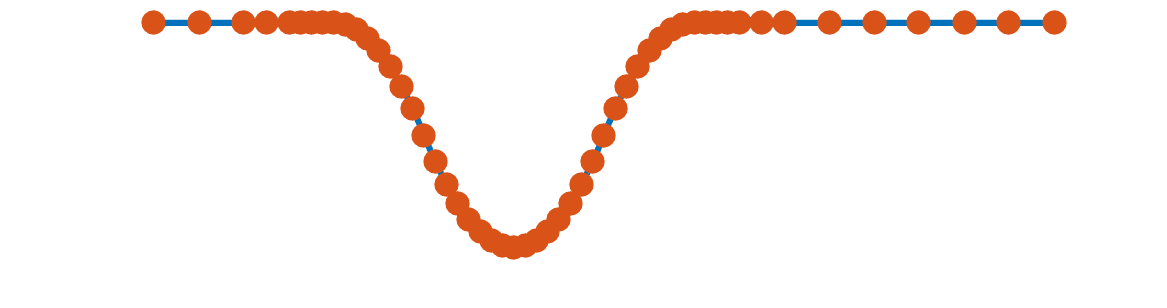
\includegraphics[width = 0.48\textwidth]{ProgramsImages/sampling-funappxg.png}
	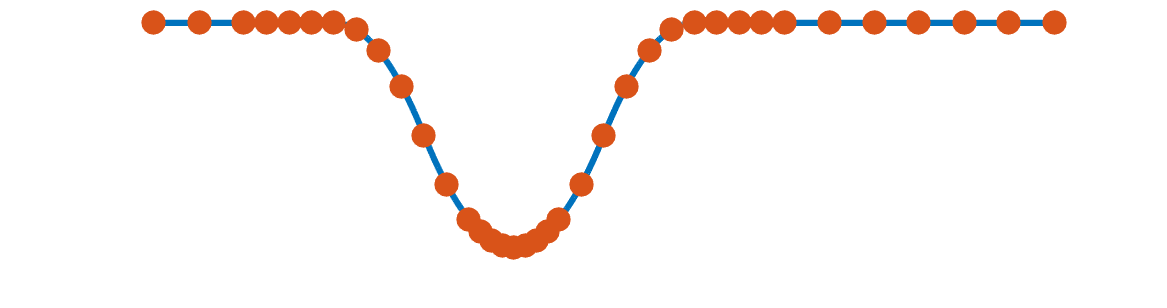
\includegraphics[width = 0.48\textwidth]{ProgramsImages/sampling-funming.png}
	
	\vspace{-2ex}
	\caption{The function data ({\color{MATLABOrange}$\bullet$}) for  locally adaptive 
	function approximation  (left) and locally adaptive optimization (right) \label{localadaptfig}}
\end{figure}


For this locally adaptive approximation algorithm 
$\cost(\fA,f,\varepsilon) = \Order\left(\sqrt{\norm[1/2]{f''}/\varepsilon} \right)$ \cite{ChoEtal17a}, 
where 
$\norm[1/2]{\cdot}$, the $1/2$-quasinorm, is weaker than the sup-norm.  This is  
asymptotically the same cost as for the best possible algorithm for this problem. In contrast, 
our older globally adaptive function approximation algorithm in \cite{HicEtal14b} has a 
computational cost of $\Order\left(\sqrt{\norm[\infty]{f''}/\varepsilon} \right)$.  For a somewhat 
spiky, but reasonable, 
function inside $\cc$, the local adaption algorithm may require significantly less effort 
than a global adaption algorithm because $\norm[1/2]{f''}$ will be much smaller than 
$\norm[\infty]{f''}$.

Similar arguments to those above lead to a locally adaptive algorithm for the 
optimization problem, $\OPT$ in \eqref{probs}.  In this case, those subintervals for which the 
function is definitely greater than the minimum found so far need not be 
refined further.  Figure 
\ref{localadaptfig} (right) gives an example of the function data required.  The function is 
sampled sparsely where either $|f''(x)|$ is small \emph{or} the $f(x)$ is large.

YZ's PhD research is developing a locally 
adaptive Simpson's rule for univariate integration.  It will have higher order accuracy than Algorithm 
\ref{Trapalg} above.  

\subsubsection[QMCsec]{Globally  Adaptive Quasi-Monte Carlo (QMC) 
Cubature} \hypertarget{QMClink}{}
\label{QMCsec}
The PI, LlAJR, and DL 
have 
developed adaptive quasi-Monte Carlo algorithms for integration over the unit cube, $\Omega = 
[0,1]^d$ \cite{HicJim16a,JimHic16a}.  For multidimensional integrals over different domains, a 
transformation of variables can 
often change the domain to the unit cube.  \QMC algorithms  commonly 
choose the 
sequence of nodes, $\{\bx_i\}_{i=1}^\infty$, to be an integration lattice node sequence  or a digital 
sequence, especially the Sobol' sequence \cite{DicEtal14a}.  \QMC cubature is superior to 
independent and identically distributed Monte Carlo (\hypertarget{IIDMClink}{IID MC}) cubature 
because the nodes are more 
evenly spread throughout the domain.   Fig.\ \ref{PtsFig} illustrates this fact.

\begin{figure}[h] % MATLAB Driver: PlotPoints.m
	\centering
	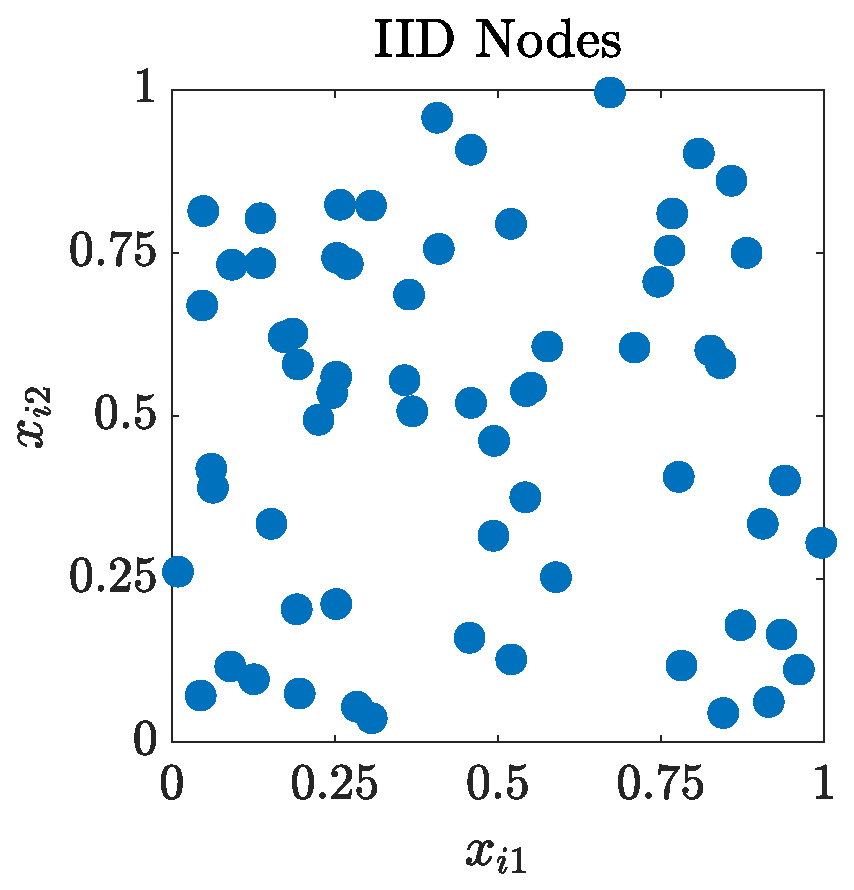
\includegraphics[width = 0.31\textwidth]{ProgramsImages/IIDPoints.eps} \quad
	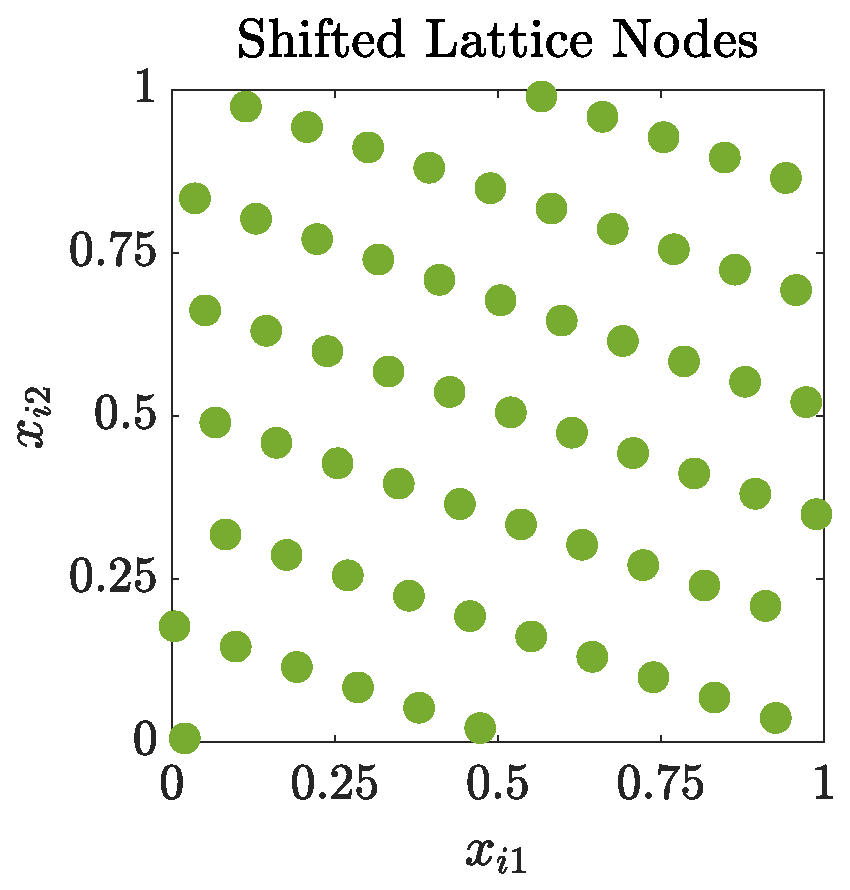
\includegraphics[width = 0.31\textwidth]{ProgramsImages/ShiftedLatticePoints.eps}  \quad
	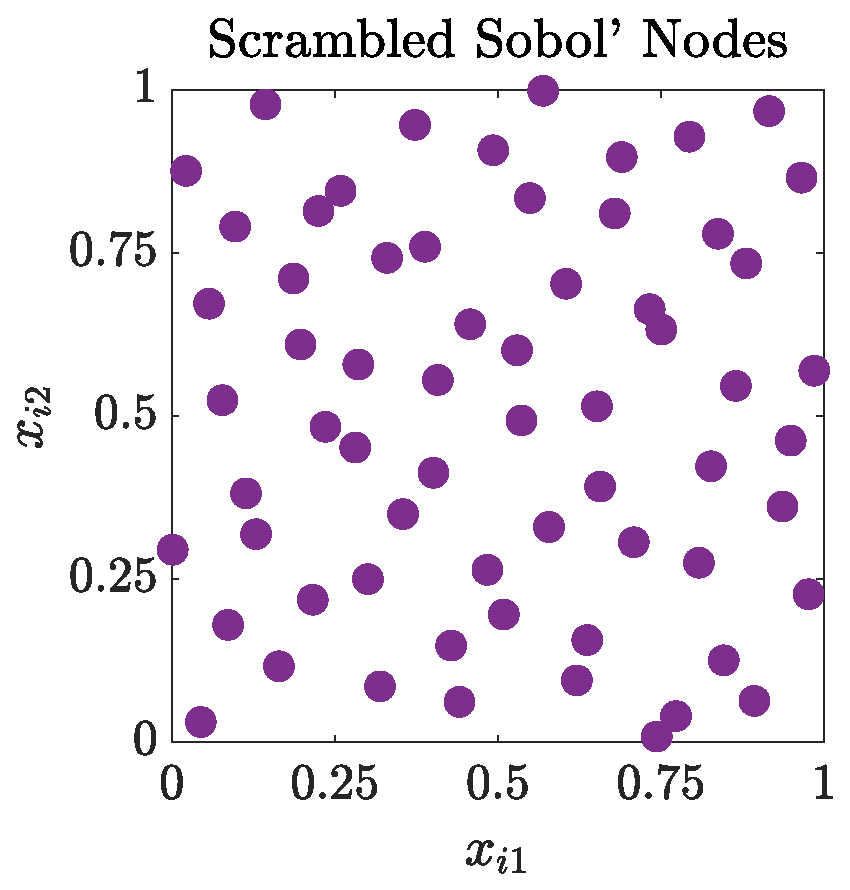
\includegraphics[width = 0.31\textwidth]{ProgramsImages/SSobolPoints.eps} 
	
	\caption{IID nodes contrasted with nodes used for QMC cubature.\label{PtsFig}}
\end{figure}

For the two kinds of \QMC sampling considered here and illustrated in Fig.\ \ref{PtsFig}, $n$ is 
commonly a power of two.  The well-known theoretical error bound for 
quasi-Monte Carlo cubature can be expressed in terms of some of the Fourier coefficients of the 
integrand \cite{DicEtal14a, DicPil10a, HicJim16a,JimHic16a, Nie92, SloJoe94}:
\begin{gather}
\nonumber
f(\bx) = \sum_{\bk \in \bbK} \hf(\bk) \phi_{\bk} (\bx),  \qquad \text{where } \hf(\bk) := \int_{[0,1]^d} 
f(\bx) \, \overline{\phi}_{\bk}(\bx) \quad \forall \bk \in \bbK, \\
\label{multiInt} \tag{M-INT} S(f): = \int_{[0,1]^d} f(\bx) \, \dif \bx, 
\qquad A_n(f) = \frac 1n \sum_{i=1}^{n} f(\bx_i), \\
\nonumber
\err_n(f) := \abs{S(f) - A_n(f)} \le \sum_{\bk \in P^\perp_n \setminus\{\bzero\}} \abs{\hf(\bk)} = : 
\oerr_n(f), \\
\nonumber
\text{Dual set: }P_n^\perp : = \{\bk \in \bbK \, \vert \, \phi_{\bk}(\bx_i) = \phi_{\bk}(\bx_1) \text{ for } 
i=1, \ldots, n \}. \\[3ex]
\nonumber
\begin{array}{ccc}
\text{\QMC Nodes} & \bbK & \phi_{\bk} \\
\toprule
\text{Shifted integration lattice sequence} & \integers^d & \text{Multivariate complex 
exponentials}\\
\text{Shifted digital sequence, e.g., Sobol' sequence} & \naturals_0^d & \text{Multivariate Walsh 
functions}
\end{array}
\end{gather}
The theoretical error bound, $\oerr_n(f)$, arises because the basis, 
$\{\phi_{\bk}\}_{\bk \in \bbK}$ is 
chosen to \emph{match} the particular \QMC nodes.  As $n \to \infty$, the dual set, $P^\perp_n$, 
loses 
elements, and $\oerr_n(f) \to 0$.

The PI and LlAJR in \cite{HicJim16a,JimHic16a} took $\oerr_n(f)$ as a starting point for their 
adaptive \QMC rules.   True Fourier 
coefficients, $\hf(\bk)$ may be approximated 
by discrete Fourier coefficients,
\begin{equation*}
\tf_n(\bk)  = \frac{1}n \sum_{i=1}^{n} f(\bx_i) \overline{\phi}_{\bk}(\bx_i).
\end{equation*}
The $n$ unique discrete Fourier coefficients can be evaluated with a computational cost of 
$\Order(n \log(n))$.  However, the index set $P^\perp_n \setminus\{\bzero\}$ contains only large 
wavenumbers, for which the discrete Fourier coefficients approximate poorly the true Fourier 
coefficients.  So, PI and LlAJR defined a cone of reasonable integrands, $\cc$, 
whose Fourier coefficients do not decay erratically.  We omit the important technical details, but 
provide an intuitive explanation.  The true Fourier coefficients of a reasonable integrand
need not decay monotonically.  But, if the average size of the true Fourier coefficients for 
moderate-sized (relative to $n$) wavenumbers is small, then the average size of the true 
coefficients for large-sized wavenumbers must also be small.  Fig.\ \ref{GoodBadWalshFig} 
illustrates an example of a reasonable function and an unreasonable function and their Fourier 
(Walsh) coefficients.  Here and in the error bound below, $\{\bk(\kappa)\}_{\kappa = 1}^\infty$ 
denotes an ordering of 
the $d$-dimensional wavenumbers in $\bbK$.

\begin{figure}[h]
	\centering
	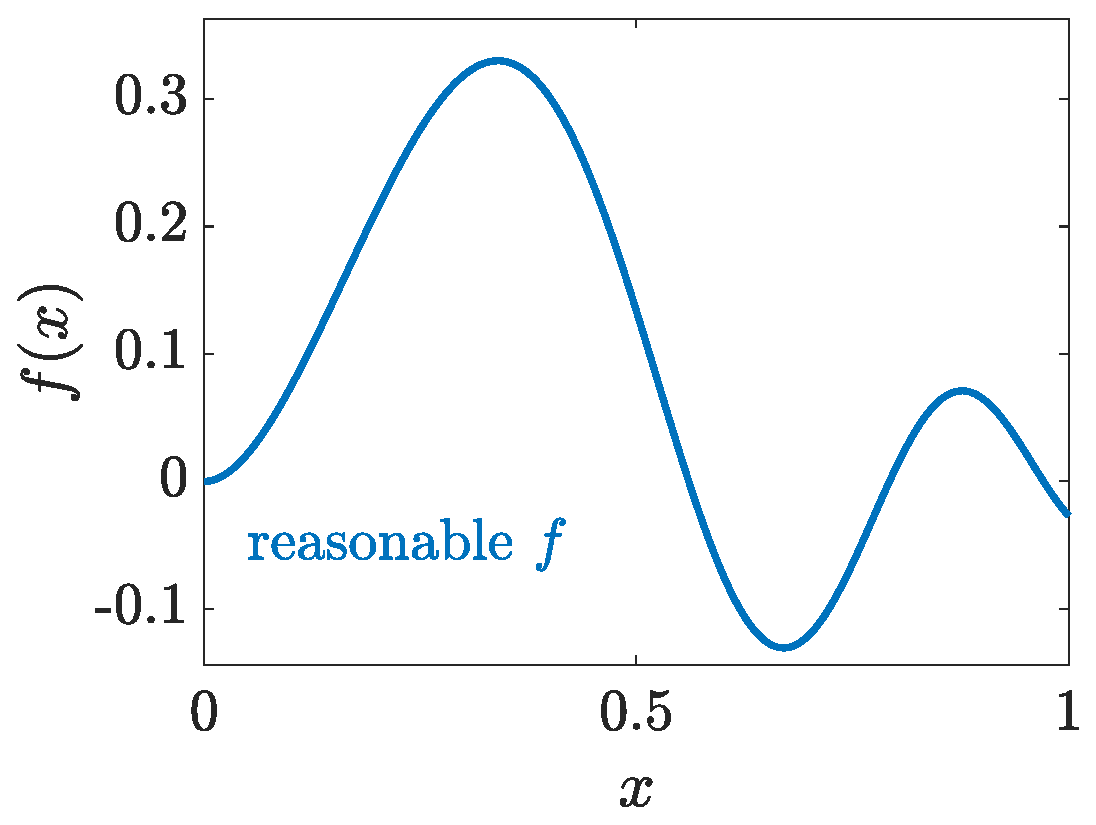
\includegraphics[width = 0.23\textwidth] 
	{ProgramsImages/FunctionWalshFourierCoeffDecay.eps} \ \ 
	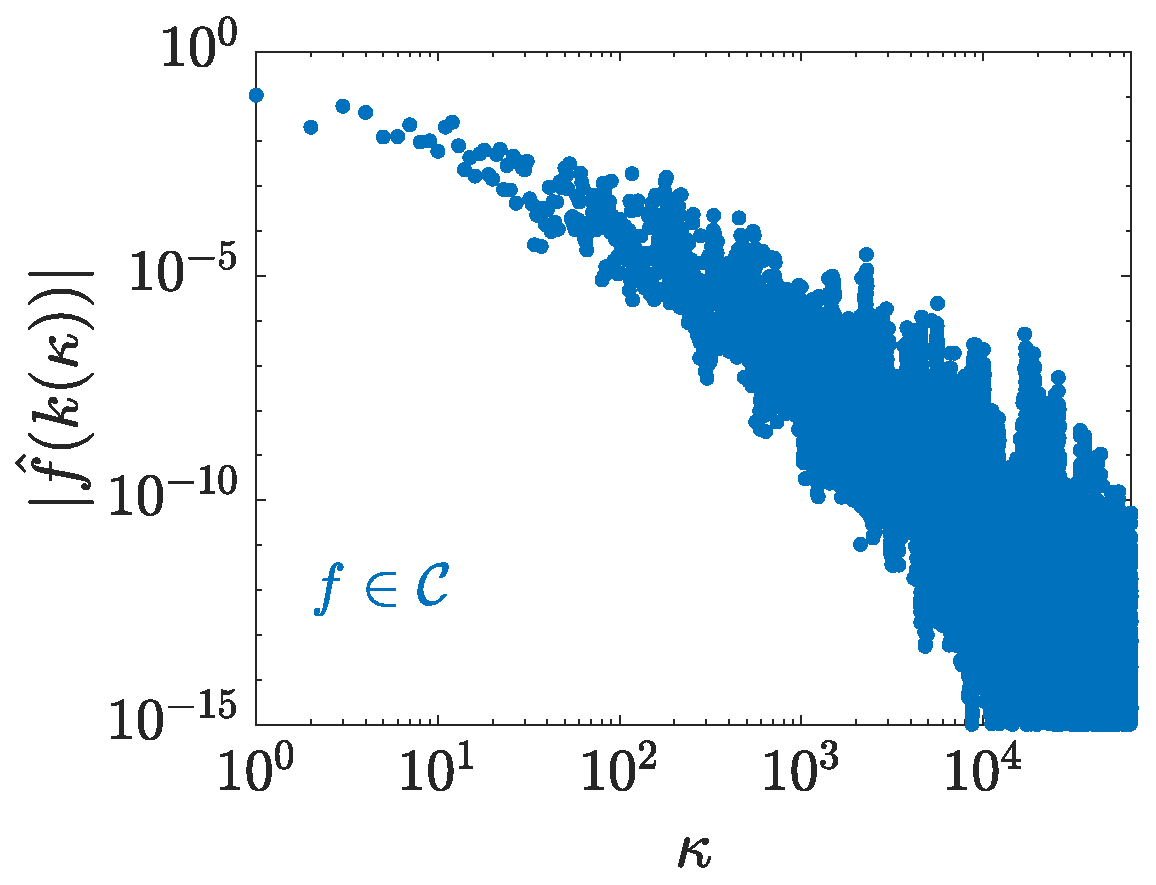
\includegraphics[width = 0.23\textwidth] 
	{ProgramsImages/WalshFourierCoeffDecay128.eps} \ \ 
	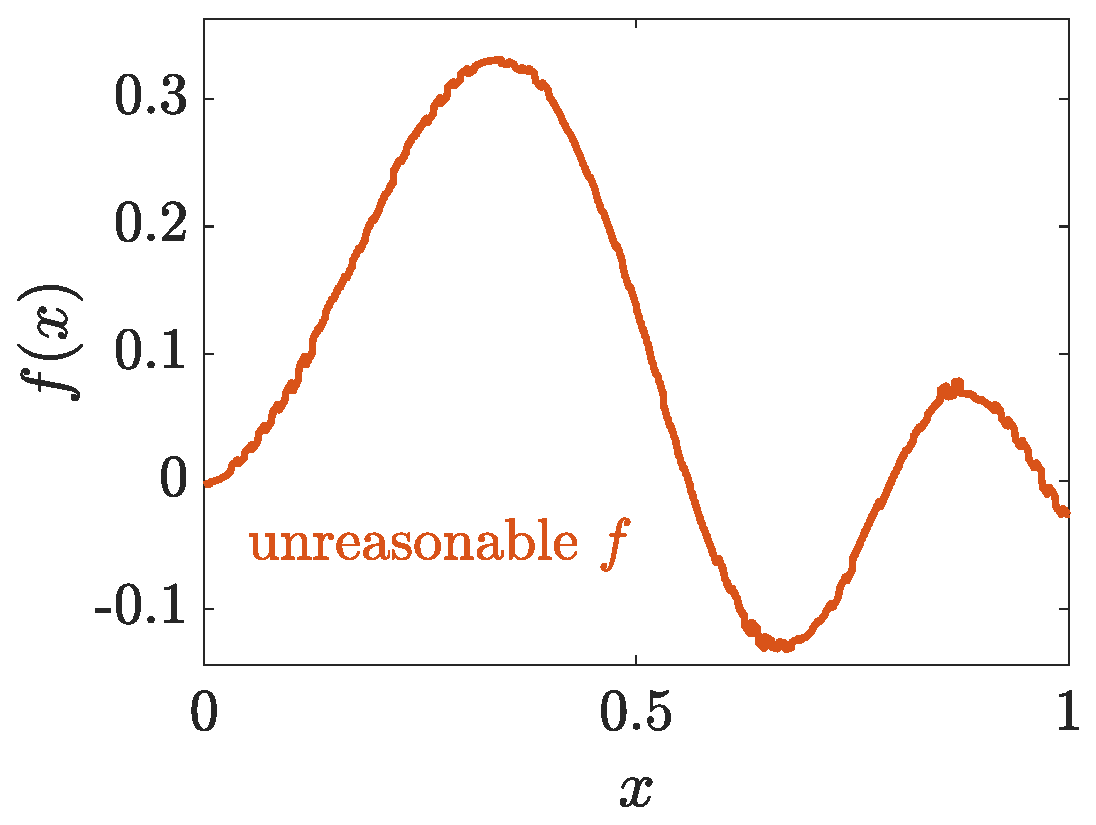
\includegraphics[width = 0.23\textwidth] 
	{ProgramsImages/FilteredFunctionWalshFourierCoeffDecay.eps} \ \ 
	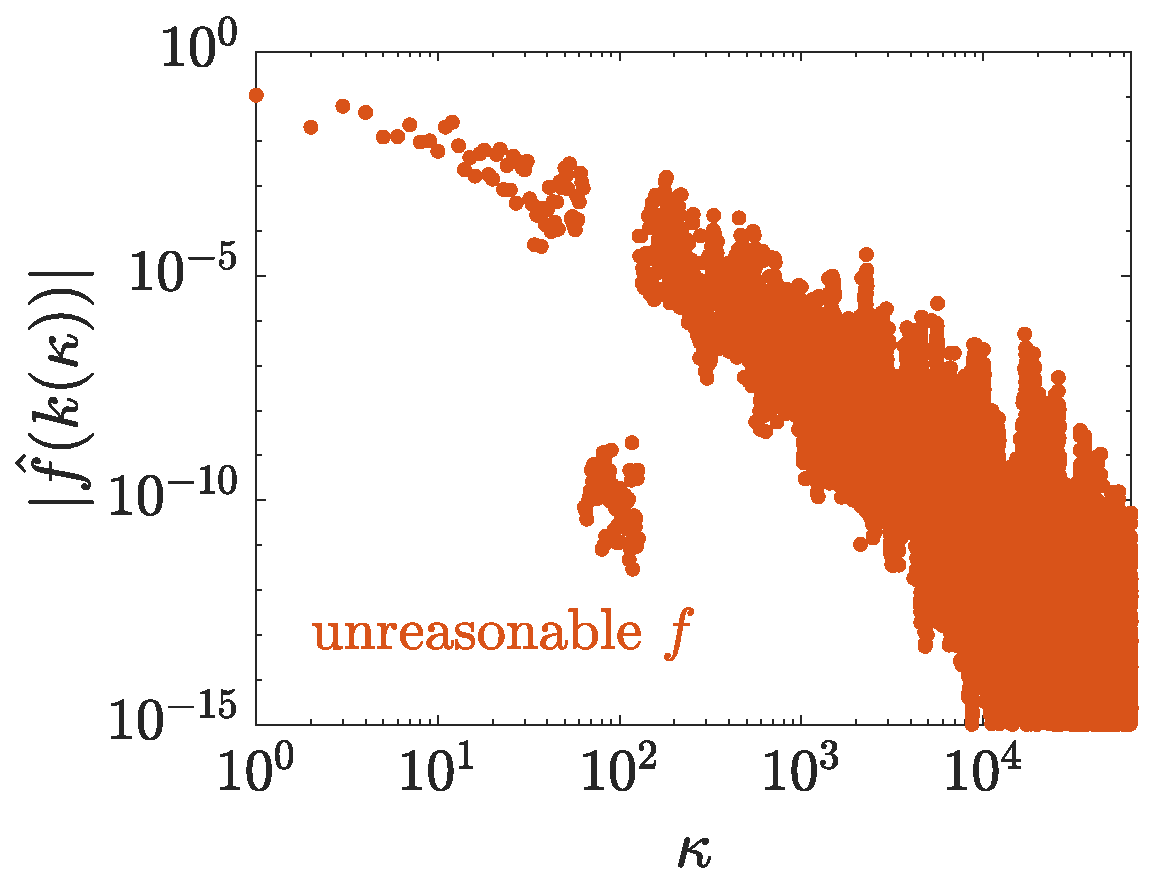
\includegraphics[width = 0.23\textwidth] 
	{ProgramsImages/WalshFourierCoeffDecayFilter.eps}
	\caption{One reasonable and one unreasonable function 
		%and their Fourier coefficients 
	\label{GoodBadWalshFig}}
\end{figure}

Under this definition of $\cc$, a 
theoretically justified, data-based error bound can be derived:
\begin{equation*}
\herr_n(f) = \fC(n) \sum_{\kappa = n/(2n_1) + 1}^{n/n_1} \abs{\tf_n(\bk(\kappa))}.
\end{equation*}
Here $\fC(n)$ is an inflation factor and $n_1$ is a power of $2$ used to define what is meant by 
``moderate-sized'' wavenumbers.  This data-driven error bound in terms of the discrete Fourier 
coefficients is used in \cite{HicJim16a,JimHic16a} to construct guaranteed adaptive \QMC cubature 
algorithms: $n$ is increased by doubling until $\herr_n(f) \le \varepsilon$.  Then choosing 
$\fA(f,\varepsilon) = A_n(f)$ satisfies  error criterion 
\eqref{errorcrit}.  

If $n$ is the final number of nodes required, the computational cost of these adaptive \QMC 
cubature algorithms  is $\Order\bigl(\$(f)n + n \log(n)\bigr)$, 
where $\$(f)$ denotes the cost of one function value.  For practical values of $n$,  $\$(f)n$ and 
$n \log(n)$ are comparable.

The PI, LlAJR, and DL have generalized the adaptive \QMC rules to accommodate control variates.  
%This means replacing the integrand $f$ by $f - \bbeta^T[\bg - S(\bg)]$, where $\bg$ is a vector 
%function whose integral, $S(\bg)$, is known exactly.  Note that $S(f - \bbeta^T[g - S(g)]) = 
%S(f)$ for any constant $\bbeta$.  The data-driven error bound now is $\herr_n(f -  
%\bbeta^T[g - S(g)])$, and the choice of $\bbeta$ can significantly decrease or increase this error 
%bound, 
%and consequently the computational cost.  
For \IIDMC cubature, a nearly optimal control variate coefficient, $\bbeta$, is 
computed by linear regression, but as pointed out by \cite{HicEtal03}, this is not necessarily the 
correct $\bbeta$ for \QMC cubature.  The PI, LlAJR, and DL provide an alternative, satisfactory 
method for 
determining $\bbeta$.
% that looks directly at $\herr_n(f -  \bbeta^T[g - S(g)])$ \cite{HicEtal17a}.

\subsubsection{Adaptive Bayesian Cubature}  \label{Bayessect} Recent research by the PI and 
JR assumes
that the integrand in the multivariate integration problem \eqref{multiInt} is an instance of a 
Gaussian 
Process with constant mean $m$, and covariance kernel, $C:[0,1]^d \times [0,1]^d \to \reals$, i.e., 
$f \sim \GP (m,C)$.  This approach to computational mathematics has been pursued by several 
scholars in the past \cite{Dia88a, OHa91a, RasGha03a, Rit00a} and has gained recent interest 
under the name \href{http://www.probabilistic-numerics.org}{probabilistic numerics}.  Under this 
approach one 
infers the mean, $m$, and the parameters defining the covariance kernel, $C$, using maximum 
likelihood estimation, and then constructs a credible interval in the Bayesian sense, $\Prob[\abs{S(f) 
- A_n(f)} \le \herr(f)] = 99\%$, where $A_n$ is the statistically best approximation to $S(f)$, and 
$\herr_n(f)$ depends on the function data and the inferred values of $m$ and $C$. 

A longstanding drawback of this approach has been the computational cost of the matrix operations 
involving the Gram matrix $\mC = \bigl(C(\bx_i,\bx_j)\bigr)_{i,j=1}^n$, which are ordinarily at least 
$\Order(n^3)$.  Attempts to overcome this cost include \cite{AniCheSte16a, ParEtal17a}.  The 
contribution of the PI and JR has been to choose families of covariance kernels with Hilbert-Schmidt 
decompositions of the form $C(\bx,\bt) = \sum_{\bk \in \bbK} \lambda_\bk \phi_{\bk}(\bx) 
\phi_{\bk}(\bt)$, where the $\phi_{\bk}$ are \emph{the same as those in the previous section}.  The 
eigenvalues $\lambda_\bk$ must be chosen so that the infinite sum has a closed form.  Such 
kernels have arisen in other contexts \cite{Hic99b,HicYue00}.  Kernels of 
this form used with the matching \QMC nodes yield Gram matrices $\mC$ for which the 
necessary vector-matrix operations can be accomplished with computational cost $\Order(n 
\log(n))$, making Bayesian cubature practical.  This work has been presented at conferences and 
as being prepared for submission for publication.

\emph{Generalized Error Criteria.}  Some practitioners may prefer the adaptive 
algorithm 
to satisfy a more general error 
criterion than \eqref{errorcrit}, e.g., 
\begin{multline}
\label{generrorcrit} \tag{G-CRIT}
\abs{\Ans(S(\vf)) - \fA(\vf,\varepsilon, \reltol) } \le \max(\varepsilon, \reltol \abs{\Ans(S(\vf))} ),  \\
 \vf: 
\Omega \to \reals^p, \ \ V: \reals^p \to \reals, \ \ S(\vf) = \bigl(S(f_1), \ldots, S(f_p) \bigr)^T, \ \  0 \le 
\reltol \le 1,
\end{multline}
where now the value sought, $\Ans(S(\vf))$, is a function the integral of $p$-vector function, 
$\vf$. Examples of situations where there the value sought is a function of several intergrals include 
Sobol' indices \cite{Sal02a} and Bayesian inference \cite{GelEtal13}.  The approximate solution is 
acceptable if it 
satisfies either an absolute error tolerance, 
$\varepsilon$, \emph{or} a relative error tolerance, $\reltol$.  The PI, LlAJR, and DL showed in 
\cite{HicEtal17a} how to use data-driven error bounds, $\abs{S(f_j) - A_n(f_j)} \le \herr_{n}(f_j)$, $j = 
1, \ldots, p$,  to 
choose an appropriate $\fA(\vf,\varepsilon, \reltol)$.  In general, the 
best approximation is \emph{not} $\Ans(A_n(\vf))$.  


\emph{Multivariate Function Approximation.}
GEF has led the effort in accurate, well-conditioned function approximation and solution of 
differential equations using reproducing kernel Hilbert space methods.  Much of his effort has been 
developing truncated Hilbert-Schmidt decomposition of the reproducing kernels using appropriate 
eigenfunctions.  For example, an expansion of the squared exponential (Gaussian) kernel using 
Chebyshev polynomials instead of Hermite polynomials has been used for the numerical solution of 
nonlinear unsteady 
convection-diffusion-reaction equations.  GEF and his collaborators have been extending 
decompositions of the Matern kernels on the half line to the entire real line, the first such analytical 
derivations.


\subsection{Broader Impacts from Previous NSF Funding} \label{prevBIsect}

\emph{Publications, Conference Participation, and Conference Organization.} This 
project has resulted in a number of publications by the PI, GEF, students, and collaborators listed at 
the beginning of this section.  We have also spoken at a number of applied mathematics, statistics, 
and computational science conferences and given colloquium/seminar talks to mathematics and 
statistics departments.  Here are some highlights.  The PI, SCC, LJ, and LlAJR recently finished an 
encyclopedia entry on adaptive Monte Carlo \cite{HicEtal18a}.  The PI co-organized the 
\href{http://cos.iit.edu/2016-spring-research-conference/}{2016 Spring Research 
Conference}, a long-running annual industrial statistics conference.   The PI gave an invited tutorial 
at the \href{http://mcqmc2016.stanford.edu}{Twelfth International 
Conference on Monte Carlo and Quasi-Monte Carlo Methods in Scientific Computing (MCQMC 
2016)} 
\cite{Hic17a}, a biennial conference for which he also serves on the steering committee.  The PI 
serves as a program leader for the Statistical and Applied Mathematical Sciences 
Institute (SAMSI) 2017--18 
\href{https://www.samsi.info/programs-and-activities/year-long-research-programs/2017-18-program-quasi-monte-carlo-high-dimensional-sampling-methods-applied-mathematics-qmc/
}{Program on Quasi-Monte Carlo and High-Dimensional Sampling Methods for Applied 
	Mathematics (\hypertarget{SAMSIlink}{SAMSI-QMC})}.   He  gave an invited tutorial 
	at the Opening Workshop, leads one of 
	the working groups, and participates in two working groups.  The PI received the 2016 Joseph F.\ 
	Traub 
	Prize for Achievement in Information-Based Complexity.
	
	
The PI's leadership in the MCQMC conferences  and \SAMSIQMC is 
	designed to bring \QMC to other areas of potential application.  One concrete example, was the 
	collaboration between the PI, LlAJR and French collaborators working in uncertainty quantification 
	that resulted in \cite{GilEtal16a, GilJim16b}.  Another example, is the collaboration of LlAJR with 
	high energy physicists at Fermilab, in the Chicago suburbs, where LlAJR was using \QMC to speed 
	up their Monte Carlo calculations.
	
\emph{\GAIL Software.} The theoretical results of this research have been implemented in 
\GAIL, the open source MATLAB library hosted on Github at 
\href{http://gailgithub.github.io/GAIL_Dev/} {\nolinkurl{gailgithub.github.io/GAIL_Dev/}}. This software 
has been implemented with input parsing, input validation, unit tests, inline documentation, and 
demonstrations.  \GAIL makes it easier for practitioners to try our new adaptive algorithms.  With the 
help of students, we are starting to port GAIL to Python and R.

\emph{Boosting the STEM Workforce.} The PI and GEF have mentored a number of 
research students associated with this project.  The main ones are mentioned at the beginning of 
this section.  Female students mentored include YD, LJ, XT, and Xiaoyang Zhao (MS IIT).   There 
have also been a 
number of 
undergraduate students who the PI, GEF, and SCC have mentored including more than a dozen 
Brazilian Science Mobility Program students in the summers of 2015 and 2016, Tanner Johnson (BS 
U 
Minnesota, MS student at U British Columbia), Tianpei Qian (BS NUS, MS student at Stanford), 
Tianci Zhu 
(female, BS IIT, MS student at NYU),  Cu Hauw Hung (BS student at Biola University, applying for 
graduate study), and Yueyi Li (female BS student at Macalester University, applying for 
graduate study).  We have also had a few high school students join us. As part of our team, all of 
these students conducted theoretical and/or practical research, some of which resulted in 
publications and new features for \GAIL.  Our students have learned how to contribute to a 
substantial, long-term software project.

The PI teaches a course on Monte Carlo methods each fall.  For the past several years students 
have been introduced to \GAIL and used it in their coursework.  \GAIL has been used to teach how 
to 
know how large $n$ must be for an \IIDMC or \QMC simulation to reach the desired accuracy 
requirement.  A number of student class projects have been devoted to improving \GAIL.

The PI was recently appointed the director of Illinois Tech's new Center for Interdisciplinary 
Scientific Computation.  In this position he has been fostering collaborative scientific computation 
research across departments by hosting matchmaking seminars and sponsoring a seed grant 
competition.


\section{Intellectual Merit of the Proposed Research} \label{secProposed}


\subsection{Higher Order Adaptive Algorithms for Univariate Problems}\label{SectUniProb}

\emph{A Theoretically Justified Alternative to MATLAB's 
\textup{\texttt{integral.m}}.} 
MATLAB's premier adaptive quadrature algorithm is based on composite high order Gaussian 
quadrature rules, so it converges much faster than our adaptive trapezoidal rule (Algorithm 
\ref{Trapalg}). However, as noted in Sect.\ \ref{TrapIllSect} and illustrated in Fig.\ 
\ref{quadfailfig}(c), 
\texttt{integral.m} can fail even for reasonable integrands, whereas our Algorithm 
\ref{Trapalg} will always succeed for reasonable integrands. The adaptive quadrature algorithms in 
the other popular scientific libraries, 
such as the NAG library, GSL, and SciPy, have the same defect as MATLAB's \texttt{integral.m}.  

YZ is already working on a locally adaptive Simpson's rule, following the ideas in Sect.\ 
\ref{localadpatsec}.  Our next step will be a 
locally adaptive high order algorithm that is competitive with MATLAB's \texttt{integral.m} but that 
has 
rigorous data-driven error bounds that will make it succeed for all reasonable 
integrands, i.e., all functions in a cone, $\cc$, to be defined.  Our goal is to provide replacement for 
MATLAB's \texttt{integral.m} and similar algorithms.  

Rather than use Gauss quadrature rules, we will likely use composite Clenshaw-Curtis quadrature, 
which is based on integrating a Chebyshev polynomial approximation to the integrand on each 
subinterval 
$[\alpha, \beta]$ of the integration interval $[a,b]$.  
Trefethen \cite{Tre08a} has pointed out that Clenshaw-Curtis quadrature is competitive with Gauss 
quadrature.  Starting with the theoretical error bounds for Clenshaw-Curtis quadrature 
\cite{BraPet11a}, we will develop a data-driven upper bound on the roughness of the 
function, 
analogous to how $\fC(2/n)\tV_n(f)$ provides  an upper bound on $\Var(f')$ in \eqref{tVdef} for 
reasonable functions.  However, rather than developing a global bound, we will develop local bounds 
as was done in \cite{ChoEtal17a}.  This will then lead to a data-driven quadrature error bounds, 
$\herr_n(f,[\alpha,\beta])$, that 
can be used to adaptively determine the sample size needed to satisfy the error criteria 
\eqref{errorcrit} or \eqref{generrorcrit}.  We will also provide an upper bound on the computational 
cost of our new algorithm and a lower bound on the computational complexity of the problem.

\emph{Locally Adaptive Optimization and Function Approximation.}
We will use a similar line of argument to that in Sect.\ 
\ref{localadpatsec} to develop a locally adaptive 
optimization algorithm of higher order convergence than the one we have constructed already.  Our 
earlier 
algorithm used piecewise linear approximations, and we expect faster convergence with piecewise 
quadratic approximations.  Again computational cost of the algorithm and computational complexity 
of the problem will be addressed.  We emphasize that while being locally adaptive, our algorithm 
finds the 
\emph{global} optimum.

We will investigate the possibility of an adaptive function approximation algorithm with higher order 
convergence than that  in 
\cite{ChoEtal17a}, again based on piecewise approximation.  However, this problem is complicated 
by the typical requirement that the 
approximation have continuous derivatives to as high an order as possible.  Such a requirement does 
not arise with integration and 
optimization.  A locally adaptive cubic spline approximation with theoretical justification may be 
possible.

\emph{Chebfun.}
Chebfun \cite{TrefEtal17a} is an elegant, popular software library that approximates functions by 
Chebyshev polynomials of 
sufficiently high degree.  These polynomials can then be used for integration, optimization, 
root-finding, and other numerical computations.  Chebfun is mainly a globally adaptive algorithm in 
that the node pattern is fixed, but the number of nodes, which corresponds to 
the the degree of the polynomial is chosen adaptively.  Although Chebfun claims to perform 
computations 
to nearly machine precision, there are no theoretical guarantees.  

We will provide a theoretical basis for Chebfun by defining a cone of reasonable functions, 
$\cc$, for which Chebfun must give the correct answer.  This will be done in a similar manner as for 
\QMC quadrature in Sect.\ \ref{QMCsec}.  The cone $\cc$ will consist of functions 
whose Chebyshev series does not decay erratically for terms with polynomial degree greater than 
some minimum value.  Functions lying outside this cone, $\cc$, will be spiky functions.   Our 
theoretical foundation for Chebfun will explain why it may or may not succeed as claimed.

\subsection{Adaptive Algorithms for Multivariate Problems}\label{SectMultiProb}

\emph{Integration over domains with unbounded dimension.} The next natural challenge for 
multivariate integration is to extend our 
globally adaptive \QMC algorithms described in Sect.\ \ref{QMCsec} to situations with infinite 
dimension:
\[
S(f) = \lim_{d \to \infty} S_d(f_d), \quad S_d(f_d):= \int_{\tOmega^d} f_d(\bx) \, \varrho_d(\bx) \, \dif 
\bx, \quad \tvarrho_d(\bx) : = \prod_{r=1}^{d} \varrho(x_r),
\]
where $f_d$ is an  approximation to $f$ that depends only on the first $d$ variables, and $\tvarrho$ 
is a probability density function on $\tOmega$.  Such 
problems arise as the expected value of a functional of the solution of a 
stochastic differential equation (SDE) using $d$ time steps.  

One way to approximate $S(f)$ is to approximate the finite 
dimensional integral $S_{d_L}(f_{d_L})$ for some large dimension, $d_L$.  However, the cost of 
evaluating $f_{d_L}(x_{d_L})$ is often proportional to $d_L$.  If $A_{n,d}$ represents an \IIDMC, 
\QMC or other cubature 
using $n$ nodes on the $d$-dimensional domain,  the true cost of approximating $S(f)$ by an 
algorithm using 
$n_L$ nodes is
$\Order(d_L n_L)$.

Two alternative methods for approximating $S(f)$ are the multi-level method (MLM) \cite{Gil15a} 
and the 
multivariate 
decomposition method (MDM) \cite{Was13b}.  (Note: the MLM for cubature is inspired by the MLM 
for solving partial differential equations, but is quite different.) The function $f$, which depends on 
$\bx=(x_1, x_2, 
\ldots) \in 
\tOmega^\naturals$, 
is decomposed into pieces that only depend on the a subset of the coordinates (see 
\cite{WanHic00b} for example):  
\begin{equation*}
f(\bx) = \sum_{\fu \subset \naturals, \abs{\fu} < \infty} f_{\fu}(\bx) = \sum_{\ell 
=1}^\infty [f_{d_\ell}(\bx) - f_{d_{\ell-1}}(\bx)], \qquad  f_d:= \sum_{\fu \subseteq \{1, 
\ldots, d\}} f_\fu, \quad f_0:= 0.
\end{equation*}
Here $\abs{\fu}$ denotes the cardinality of the set $\fu$.  This decomposition is not unique and may 
be based on convenience.  Each $f_{\fu}$ depends 
only 
on the coordinates with indices in $\fu$.  If $A_{n,d}$ represents a cubature 
using $n$ nodes on the $d$-dimensional domain, $\tOmega^d$, then the MLM and MDM cubatures 
for 
approximating $S(f)$ are \cite{Gil15a, Was13b}
\begin{gather*}
A^{\textup{MLM}}_{\bn,\bd}(f) = \sum_{\ell=1}^L A_{n_l,d_l}(f_{d_\ell} - f_{d_{\ell-1}}), \quad \bn = 
(n_\ell)_{\ell = 1}^L, \ \bd = 
(d_\ell)_{\ell = 1}^L, \quad \cost(f,A^{\textup{MLM}}_{\bn,\bd}) = \Order\left (\sum_{\ell=1}^L d_\ell 
n_\ell \right), \\
A^{\textup{MDM}}_{\bn,\fU}(f) = \sum_{\fu \in \fU} A_{n_{\fu},\abs{\fu}}(f_{u}), \quad \bn = 
(n_\fu)_{\fu \in \fU}, \ \bd = 
(d_\fu)_{\fu \in \fU}, \quad \cost(f,A^{\textup{MDM}}_{\bn,\bd}) = \Order\left (\sum_{\fu \in \fU} d_\fu 
n_\fu\right).
\end{gather*}
At first glance, these costs may look greater than the $\Order(d_L n_L)$ cost of the single-level 
cubature 
$A_{n_L,d_L}(f)$.  However, the MLM and MDM are actually more 
economical for commonly occurring integrals when the goal is meeting a fixed error tolerance.   The 
low dimensional cubatures (small $d_\ell$ or $\abs{\fu}$) require 
larger numbers of nodes ($n_\ell$ or $n_{\fu}$),  
but the higher dimensional cubatures (large $d_\ell$ or $\abs{\fu}$) actually require fewer numbers 
of nodes.  In contrast, the single-level cubature requires a large number of nodes for a high 
dimension.

Adaptive MLMs constructed so far are based on heuristics.  The MDM is still in the early stages of 
practical application.  In theory, for nice enough integrands the costs of both methods for satisfying 
\eqref{errorcrit} are proportional to the costs of the finite-dimensional cubatures used, i.e., 
$\Order(\varepsilon^{-2})$ for \IIDMC and $\Order(\varepsilon^{-1+\delta})$ for \QMC.  The 
challenge 
in constructing a 
\emph{theoretically sound} adaptive algorithm is determining good choices 
of the dimension vector $\bd$ for MLM or the set of sets of important coordinate directions, $\fU$, 
for MDM.
These must be chosen so that (i) the error due to ignoring some pieces of the integrand is negligible 
and (ii) the total cost of the cubatures is small. 
Once  $\bd$ or $\fU$ are fixed, our adaptive cubatures in Sect.\ \ref{QMCsec} can be used to 
determine the vector $\bn$ needed to meet the error criterion.  We propose to develop sound 
adaptive cubatures $\fA^{MLM}$ and $\fA^{MDM}$ for infinite dimensional integration satisfying the 
error criteria \eqref{errorcrit} and 
\eqref{generrorcrit}.  The PI's familiarity with the MLM \cite{HicMGRitNiu09a, NiuHic09a, 
NiuHic09b} will facilitate this task.

\emph{Generalized Error Criterion for \IIDMC.}  LJ developed a theoretically justified \IIDMC 
algorithm satisfying a hybrid error criterion encompassing both absolute and relative error in her PhD 
thesis \cite{Jia16a}.  However, her error criterion is not as general as \eqref{generrorcrit} in that it 
does not allow the desired answer to be a function of several integrals.  We will generalize LJ's work 
to 
cover this case.  There are challenges working in this setting because the algorithm is random and 
so the error criterion should be satisfied with some confidence level $1- \alpha$.  The eventual 
$n$ required is determined sequentially by increasing it and then re-determining whether the 
generalized 
error tolerance---which depends on the unknown answer---is met.  Each step in 
the sequential algorithm must proceed 
with a 
higher confidence so that the target confidence level can be reached.

We  do not yet have a bound on the computational complexity in this randomized setting for 
multivariate integration.  We are discussing this problem with collaborators and hope to discover the 
answer.

\emph{Bayesian cubature.} The ideas being worked out by JR for his PhD thesis as described in 
Sect.\ \ref{Bayessect} are complete for the lattice node \QMC sampling, but not yet for the digital 
sequence node \QMC sampling.  In particular, we expect that smoother kernels and higher order 
nets 
will lead to higher order adaptive cubature methods.


\emph{Function approximation using matching kernels and sampling schemes.}
The Bayesian cubature framework may also be adapted to function approximation.  This approach is 
known as kriging or Gaussian process modeling in the statistics literature \cite{RasWil06a,Ste99} 
and is known as meshfree/radial basis function 
approximation in the 
numerical analysis literature \cite{Fas07a,FasMcC15a,Wen05a}.  Although the theory is 
well-developed, the computational cost of operations involving the $n \times n$ Gram matrix, 
$\mC$, mentioned in Sect.\ \ref{Bayessect} can be prohibitive.  

We will employ the \QMC node sequences with their well-matched kernels for multivariate function 
approximation, similar to what  we 
have already found successful for cubature.  We will 
develop theoretically justified adaptive algorithms and bounds on their computational costs.  
Because the theory of \QMC node sequences for function approximation using kernels is 
under-developed, there 
is much work to be done.

\subsection{Adaptive Algorithms for Problems with Expensive Function Values} 
\label{SectExpensive}
The previous two subsections have considered the situation where the time cost of a function value, 
$f(\bx)$, is comparable to the cost of a floating point operation, or at worst, the cost of $d$ floating 
point 
operations, where $d$ is the dimension.  In this section we consider problems where the time cost 
of a function value is more expensive than the cost of $n^p$ floating point operations for any 
practical $p$.  A climate model may take hours or days to complete one run.  A simulation of the 
future performance of a financial portfolio may take hours.  The outputs from simulations like these 
depend on parameters, $\bx \in \reals^d$, whose values are uncertain or whose effect 
on the output, $f(\bx)$ one needs to understand.

We want to know under what situations one can integrate or approximate a function using only
$\Order(d)$ function values, because this is the minimum number required to understand how each 
scalar input affects the output.  Furthermore, we want to develop adaptive algorithms for function 
approximations.  These surrogate models will facilitate cheap ``what-if'' explorations. 

The three-volume series of monographs \cite{NovWoz08a,NovWoz10a,NovWoz12a} summarizes a 
huge body of work on the \emph{tractability} of integration and function approximation 
problems, essentially, under what conditions the computational cost of satisfying \eqref{errorcrit} is 
$\Order(d^q \varepsilon^{-p})$ as $d \to \infty$.  We want $q=1$.  The PI has contributed to this 
literature 
\cite{FasHicWoz12b,HicSloWas03a,HicSloWas03b,HicSloWas03c,HicSloWas03e,HicWasWoz06a,HicWoz00b,WanHic00b,YueHic04a,YueHic05a,ZhoHic15a}.
  It is 
common to consider weighted tensor product 
spaces of input functions, such as the following Hilbert space with the decomposition notation 
adopted 
in Sect.\ \ref{SectMultiProb}:
\begin{equation*}
\calf := \left\{ f : [0,1]^d \to \reals \, \Big \vert \norm[\calf]{f}^2 := \!\!\!\sum_{\fu \subseteq \{1, 
\ldots, d\}} 
\frac{1}{\gamma_{\fu}^2}\int_{[0,1]^d}\abs{\frac{\partial^{\abs{\fu}}f_{\fu}}{\partial \bx_\fu}(\bx_u)}^2 
\,  
\dif \bx
\right\}.
\end{equation*}
The coordinate weights, $\bigl(\gamma_{\fu} \bigr)_{\fu \subseteq \{1, \ldots, d\}}$, indicate the 
importance of the subsets of coordinate indices.  The smaller $\gamma_{\fu}$ is, the less influential 
$f_\fu(\bx)$ is assumed to be on $f(\bx)$.  In other words, for $f$ with moderate sized norm, 
$f_\fu$ 
must be small if $\gamma_{\fu}$ is small. The literature cited above provides necessary and 
sufficient conditions 
guaranteeing that integration and function approximation are tractable for weighted spaces like the 
one above.  For product weights, $\gamma_{\fu} = \prod_{r \in \fu} \gamma_r$, tractability is 
guaranteed  
if $\gamma_{r} \to 0$ quickly enough as $r \to \infty$.  Algorithms can be constructed whose 
computational cost depend reasonably on dimension.

For some applications one knows how to order the coordinates in roughly order of decreasing 
importance, but for the applications we have in mind, such an ordering does not exist.  It must be 
discovered by evaluating the function.  Only then, can the 
tractability literature can be applied only after an initial probe of the function indicates 
which coordinates are more important.

Two of the \SAMSIQMC working groups that the PI belongs to are exploring how to
place an initial set 
of nodes evenly to uncover the important coordinate directions of $f$, followed by node 
placement that favors the important 
coordinate directions to approximate $f$ well.  We expect the existing literature plus the new ideas 
arising from the working groups will set us on a path to solving this problem.

\section{Broader Impacts of the Proposed Research}\label{SectBroad}


\subsection{Contributions to Training, Mentoring and Other Human Resource Developments}
The PI runs a weekly research group meeting comprised of long-term and short-term student 
collaborators, 
visitors, the curious, and special guests.  Ongoing work in early or polished stages is shared.  Papers 
of other authors are presented.  Mentoring takes place during these meetings as well as individually.

\emph{Providing Research Experiences for Undergraduate and High School Students.} Students 
should be introduced to research before graduate school so that they can learn how to 
discover the unknown, something that is not necessarily taught in the classroom. We request funds 
to 
support two summer REU students per year.  Our small REU program has established some visibility 
and is prompting inquiries from prospective participants well before we 
even announce our latest 
offerings. As in the past, we expect the NSF funds will serve as a catalyst for funds to 
support additional summer students. In choosing REU students we will make a deliberate effort to 
build 
a diverse research environment by targeting female and underrepresented minority students as well 
as students from less research-focused institutions (see Sect.~\ref{prevBIsect}). We will also 
welcome well-prepared high school students to join our research group.

\emph{Preparing Students for Academic Careers.} Mentoring is a multi-faceted and 
potentially long-term process continuing even after the mentee has moved on from Illinois Tech.  
Our PhD students gain experience both research and mentoring the younger students in our 
research group.  We 
continue contact with many of our former students in academia.  In particular we continue to have 
collaborations with YD, Qi Ye, and Yiou Li.  We will continue to help our students prepare for 
academic careers and continue mentoring them after they leave Illinois Tech.

\emph{Preparing Students for Industry Careers.}
We also help current students land 
competitive jobs in the business world. Our training in the areas of computation and software 
development gives our students the needed edge in comparison to other mathematics 
graduates. For example, LlAJR and XZ are working in the financial services industry and  LJ is 
working in marketing analytics.  All of them are developing and testing quantitatively sophisticated 
and computationally intensive models.

\emph{Supervising Visitors.}
Both the PI and the Co-PI have strong connections to East Asia.  We have hosted several long-term 
self-funded visitors in the past and plan to do so in the future.

\emph{Giving Tutorials and Invited Lectures.}
We will continue providing lectures to students at various stages in their careers, ranging from high 
school to graduate school. These encourage students to enter STEM and encourage STEM students 
to engage in research.


\subsection{Contributions to Resources in Research, Education and the Broader Society} 
\label{BroaderTwoSec}

The research we propose straddles mathematics, statistics, theoretical computer science, and 
application 
areas.  The two PIs have complementary strengths that facilitate this interdisciplinary research.  FJH 
has expertise in \QMC methods, kernel-based methods, information-based complexity 
theory, and experimental design. SCC has expertise in computer science and applications.  Our 
expertise provides both an obligation and an opportunity to interact with a number of diverse 
communities. We envision the following contributions:

\emph{Disseminating Research}
The research supported by this grant will result in publications in peer-reviewed journals in applied 
mathematics, computer science, statistics, and science/engineering. These 
journals will include both those that emphasize theory and those that emphasize applications.

\emph{Promoting Cones.} The idea of guaranteed, adaptive algorithms via cones of reasonable input 
functions 
has broad potential application.  We will continue to promote this idea among numerical analysts 
who 
develop new algorithms and analyze their computational costs, as well as among information-based 
complexity theorists who analyze the lower bounds on the complexity of numerical problems.  A 
posteriori error analysis for finite element analysis may be an area where we can contribute since 
this involves quadratures and cubatures.

\emph{Bridging Applied Mathematics and Statistics.}
This project touches on topics that are of interest to the statistics community: kriging, Monte Carlo 
methods, and design of experiments.  We have and will continue to engage the statistics community 
by speaking a their conferences and departmental colloquia.  For example, the PI visited the 
statistics group at Georgia Tech earlier this year, and the PI is also engaging statisticians and 
applied mathematicians through the \SAMSIQMC program.

\emph{Organizing and Presenting at Conferences.}
We and our students involved in this project will present our results at a variety of conferences and 
workshops.  These include: (i) specialized meetings focusing on approximation theory, complexity, 
experimental design, and Monte Carlo methods; (ii) the national meetings of AMS, SIAM, and the 
statistical societies; and (iii) conferences devoted to application areas.  We are frequently invited to 
speak at such conferences, which will give our results a prominent hearing. We will also continue to 
organize specialized conferences or minisymposia within larger conferences.

\emph{Writing Survey Papers.}
The PIs will continue their practice of writing tutorial, survey, and encyclopedia articles.  These will 
make our findings accessible to a wider audience.

\emph{Refreshing Course Syllabi.}
MATH 565 (Monte Carlo Methods in Finance), taught every fall by FJH, has incorporated our new 
results on guaranteed (quasi-)Monte Carlo multivariate integration. In the future it will include our 
new results on our guaranteed MLM and MDM (see Sect.\ \ref{SectMultiProb}).

As noted in Sect.\ \ref{TrapIllSect}, current texts propagate poor practices for 
adaptive quadrature.  We will urge numerical analysis textbook authors and educators to change the 
way that error estimation is taught based on our recent and proposed work.  These ideas will also 
enter our more traditional numerical analysis courses such as MATH 350 (Intro to Computational 
Math).  SCC and FJH will continue to develop MATH 573 (Reliable Mathematical Software) as a 
valuable course for our own students and an example that we wish to propagate to other 
universities.

\emph{Creating Software and Collaborating with Software Developers.}
We will continue to develop \GAIL \citep{ChoEtal17b} (now up to version 2.2).  The \GAIL software 
will 
serve the wider community that relies on numerical approximation and integration algorithms.  It will 
also demonstrate how adaptive algorithms ought to be implemented, which we hope will inspire and 
inform those working on adaptive algorithms for other mathematical problems.  We will involve 
students in porting \GAIL to other platforms, such as Python, R, and Julia.  We expect our 
new algorithms to be incorporated into widely used numerical packages, as was done for our 
algorithm in \cite{HonHic00a} by \Matlab \citep{MAT9.3} and NAG \citep{NAG23}.  We will continue 
to discuss with software developers about good practices for adaptive algorithms.

\emph{New Applications of \QMC.}
The application of \QMC has focused on a few areas, such as financial modeling and computer 
graphics, but there is 
potential for much wider application.  LlAJR has collaborated with Fermilab implementing \QMC 
algorithms, and we plan to continue.    New applications of \QMC are arising from \SAMSIQMC that 
we plan to pursue.  Presently, KZ is exploring how to use \QMC to more efficiently perform Bayesian 
inference.



\newpage
\clearpage
%\pagenumbering{arabic}
\setcounter{page}{1}

\bibliographystyle{spbasic.bst}


{\renewcommand\addcontentsline[3]{} 
\renewcommand{\refname}{{\Large\textbf{References Cited}}}                   %%
\renewcommand{\bibliofont}{\normalsize}

\bibliography{FJH23,FJHown23}}
\end{document}
